% Some notes / rules:
% - Things marked \apw{} are APW's requests for Katie
% - Things marked \todo{} can be addressed by anyone

\documentclass[twocolumn]{aastex631}

% Packages
\usepackage{microtype}  % ALWAYS!
\usepackage{amsmath}
\usepackage{amsfonts}
\usepackage{amssymb}
\usepackage{multirow}

\definecolor{pink}{RGB}{232,132,161}
\newcommand{\kc}[1]{\textcolor{pink}{\textbf{#1}} }

\newcommand{\mlg}{\ensuremath{M_{\rm LG}}}
\newcommand{\mmto}{\ensuremath{M_{\rm M31}}}
\newcommand{\mmw}{\ensuremath{M_{\rm MW}}}
\newcommand{\vtan}{\ensuremath{v_\textrm{tan}}}
\newcommand{\vrad}{\ensuremath{v_\textrm{rad}}}
\newcommand{\mud}{\ensuremath{\mu_\delta}}
\newcommand{\mua}{\ensuremath{\mu_\alpha^*}}
\newcommand{\bov}{\ensuremath{\boldsymbol{v}}}
\newcommand{\pos}[2]{\ensuremath{\boldsymbol{x}_{\rm #1 \to #2}}}
\newcommand{\vel}[2]{\ensuremath{\bov_{\rm #1 \to #2}}}
\newcommand{\mwbary}{\ensuremath{\textrm{MW}_\textrm{bary}}}
\newcommand{\mwouter}{\ensuremath{\textrm{MW}_\textrm{outer}}}
\newcommand{\mwdisk}{\ensuremath{\textrm{MW}_\textrm{disk}}}
\newcommand{\reflabel}[1]{\ensuremath{^{\mbox{\scriptsize{#1}}}}}

% Style tweaks
% \renewcommand{\twocolumngrid}{\onecolumngrid}
% \setlength{\parindent}{1.1\baselineskip}
% \sloppy\sloppypar\raggedbottom\frenchspacing

%%%%%%%%%%%%%%%%%%%%%%%%%%%%%%%%%%%%%%%%%%%%%%%%%%%%%%%%%%%%%%%%%%%%%%%%%%%%%%%%
\shorttitle{Updated Local Group Mass from Timing Argument}
\shortauthors{Chamberlain et al.}

%%%%%%%%%%%%%%%%%%%%%%%%%%%%%%%%%%%%%%%%%%%%%%%%%%%%%%%%%%%%%%%%%%%%%%%%%%%%%%%%
\graphicspath{{./}{figures/}}
% Missions
\newcommand{\project}[1]{\textsl{#1}}

% Packages / projects / programming
\newcommand{\package}[1]{\textsl{#1}}
\newcommand{\acronym}[1]{{\small{#1}}}
\newcommand{\github}{\package{GitHub}}
\newcommand{\python}{\package{Python}}
\newcommand{\astropy}{\package{Astropy}}

% Stats / probability
\newcommand{\given}{\,|\,}
\newcommand{\norm}{\mathcal{N}}
\newcommand{\pdf}{\textsl{pdf}}

% Maths
\newcommand{\dd}{\mathrm{d}}
\newcommand{\transpose}[1]{{#1}^{\mathsf{T}}}
\newcommand{\inverse}[1]{{#1}^{-1}}
\newcommand{\argmin}{\operatornamewithlimits{argmin}}
\newcommand{\mean}[1]{\left< #1 \right>}

% Non-scalar variables
\renewcommand{\vec}[1]{\ensuremath{\bs{#1}}}
\newcommand{\mat}[1]{\ensuremath{\mathbf{#1}}}

% Unit shortcuts
\newcommand{\Msun}{\ensuremath{\mathrm{M}_\odot}}
\newcommand{\Mjup}{\ensuremath{\mathrm{M}_{\mathrm{J}}}}
\newcommand{\kms}{\ensuremath{\mathrm{km}~\mathrm{s}^{-1}}}
\newcommand{\pc}{\ensuremath{\mathrm{pc}}}
\newcommand{\kpc}{\ensuremath{\mathrm{kpc}}}
\newcommand{\Mpc}{\ensuremath{\mathrm{Mpc}}}
\newcommand{\kmskpc}{\ensuremath{\mathrm{km}~\mathrm{s}^{-1}~\mathrm{kpc}^{-1}}}
\newcommand{\dayd}{\ensuremath{\mathrm{d}}}
\newcommand{\yr}{\ensuremath{\mathrm{yr}}}
\newcommand{\Kel}{\ensuremath{\mathrm{K}}}

% Misc.
\newcommand{\bs}[1]{\boldsymbol{#1}}

% Astronomy
\newcommand{\DM}{{\rm DM}}
\newcommand{\feh}{\ensuremath{{[{\rm Fe}/{\rm H}]}}}
\newcommand{\df}{\acronym{DF}}

% TO DO
\newcommand{\todo}[1]{{\color{red} TODO: #1}}
\newcommand{\apw]}[1]{{\color{green} APW says: #1}}

% Projects
\newcommand{\gaia}{\textsl{Gaia}}
\newcommand{\gaiadr}{\textsl{Gaia}~\acronym{EDR3}}


% Affiliations
\newcommand{\affuofa}{University of Arizona, 933 N. Cherry Ave,
    Tucson, AZ 85721, USA}
\newcommand{\affcca}{Center for Computational Astrophysics, Flatiron Institute,
    Simons Foundation, 162 Fifth Avenue, New York, NY 10010, USA}
\newcommand{\affedinb}{Institute for Astronomy, University of Edinburgh,
    Royal Observatory, Blackford Hill, Edinburgh EH9 3HJ, UK}
\newcommand{\affparis}{Institut d'Astrophysique de Paris,
    98 Bis Blvd Arago 75014 Paris, France}

%% This is the end of the preamble.  Indicate the beginning of the
%% manuscript itself with \begin{document}.

\begin{document}

\title{
    A timing argument mass for the Local Group accounting for the
    Milky Way--LMC reflex motion
}

\author[0000-0001-8765-8670]{Katie~Chamberlain}
\affiliation{\affuofa}
\affiliation{\affcca}

\author[0000-0003-0872-7098]{Adrian~M.~Price-Whelan}
\affiliation{\affcca}

% TODO: Alphabetical ok?
\author[0000-0003-0715-2173]{Gurtina Besla}
\affiliation{\affuofa}

\author[0000-0002-6993-0826]{Emily C. Cunningham}
\affiliation{\affcca}

\author[0000-0001-7107-1744]{Nicol\'{a}s Garavito-Camargo}
\affiliation{\affcca}

\author{Jorge Pe\~{n}arrubia}
\affiliation{\affedinb}

\author[0000-0003-1517-3935 ]{Michael Petersen}
\affiliation{\affparis}

% TODO: Any other authors??

\begin{abstract}
    % \textbf{Context}
    The total mass of the Local Group (LG) is a fundamental quantity that
    enables interpretation of the orbits of its constituent galaxies and is
    needed to place the LG in a cosmological context.
    One of the few methods that enables inferring the total mass directly is the
    ``Timing Argument,'' which models the relative orbit of the Milky Way (MW)
    and M31.
    \todo{maybe this should be something closer to "previous encounters + mergers with dwarf galaxies have imparted a reflex motion of the disk, especially the LMC" ? }
    However, recent models of stellar tracers in the outer MW halo have shown
    that the inner MW and disk are moving with respect to the outer halo, likely
    because of the infall of the Large Magellanic Cloud, thus biasing past
    Timing Argument measurements that do not account for this motion.
    % \textbf{Aims}
    % \textbf{Methods}
    Here, we measure the total LG mass using a Timing Argument model that
    incorporates this measured ``travel velocity'' of the MW disk using several
    different compilations of recent kinematic measurements of M31.
    % \textbf{Results}
    We generally find lower LG masses than past Timing Argument results and
    measure a consistent (between datasets) total mass of
    $4.5^{+0.8}_{-0.6}\times 10^{12}~\Msun$ using the travel velocity $32 \pm
    4~\kms$ measured in \citet{Petersen2021}.
    Measurements of the travel velocity with more distant tracers could yield
    even larger values, which would further decrease the inferred LG mass.
    Additionally, we find that future data releases from \emph{Gaia} will lead 
    to more precise measurements
    of M31's proper motion that will improve the precision of Timing Argument
    mass constraints by a factor of $\sim2$.
    % \textbf{Conclusions}
    Thus, this newly measured travel velocity implies a lower LG mass than from 
    a system with a static MW halo and must be considered in future dynamical 
    studies.
    % The Timing Argument remains one of few ways to measure the Local Group
    % mass independent of the masses of the individual component galaxies, but
    % it is clear that the dynamical impact of the MCs must be accounted for when
    % using these techniques.

\end{abstract}

\section{Introduction}
\label{sec:intro}
% \textbf{Importance of local group mass and measuring it}
\todo{Review references - any obvious missing?}
\todo{do we need to rethink the language of "Milky Way disk" vs. inner MW halo?}
\todo{need to specify the parameters of the travel velocity that we are using somewhere!}
The total mass of the Local Group is an important quantity in many local
cosmological and Milky Way (MW) applications.
For example, it is used to identify analogous halos in cosmological simulations
and thus allows comparing host galaxy and satellite galaxy number counts and
properties \citep[e.g.,][]{Patel2017a, Marinacci:2017, Dooley2017, Besla2018,
Patel2018, Garrison-Kimmel:2019a, Garrison-Kimmel:2019b, Sawala2022}.
It is also used to turn the kinematics of Local Group
galaxies into orbital histories \citep[e.g.,][]{Peebles:2017}, which is used to
interpret their gas content \citep[e.g.,][]{Fillingham:2018,Putman:2021} and
star formation histories \citep[e.g.,][]{Tolstoy:2009}.
However, as most of the mass in the Local Group is in dark matter distributed
over megaparsec scales, it is difficult to directly measure its total mass.

Given its utility in studies of the local universe, several methods have been
used to dynamically infer the mass of the Local Group.
Many of these techniques determine the individual masses of the MW and M31
independently \citep[e.g.][]{Watkins2010, Diaz2014, Patel2018, Eadie:2019,
Fritz:2020, Deason:2021, Wang:2022}, often via the dynamics of their satellites
and stellar streams, then combine them to get an estimate of the total LG mass.
Other techniques aim to more directly measure the mass of the Local Group en
masse, for example looking for Local Group analogs in cosmological simulations
based on stellar mass and kinematic criteria \citep[e.g.,][]{Zhai2020}, or by
studying the kinematics of Local Volume galaxies
\citep[e.g.,][]{Penarrubia2014}.
One of the earliest methods utilized in this vein is the ``Timing Argument,''
which uses the fact that the local group galaxies (most often the MW and M31)
are bound and approaching pericenter in their relative orbit, but must have been
close enough over cosmic time to not be pulled apart by the Hubble flow. We
summarize the relevant details of the Timing Argument method in
Section~\ref{sec:timingarg}

The Timing Argument (using the MW and M31) uses the observed kinematics of M31
to model the relative orbit of the two galaxies as a Keplerian orbit.
Assuming Keplerian dynamics enables dynamically measuring the total mass of the
MW and M31 with analytic expressions for all relevant kinematic quantities
because of the simplicity of the two-body equations of motion.

\kc{\begin{itemize}
  \item here, talk about how the assembly history of the MW and M31 has an impact on the dynamics of the pair. In the past, the impact of the LMC on the change in MW+LMC barycenter has been studied by Penarrubia et al. 
  \item Talk about predictions of reflex motion of disk -- how the LMC has pulled on the disk of the MW and about the predictions etc from that. (would solid body stuff have to go here?) Recent work by Benisty 
  \item Introduce travel velocity (the instantaneous measurement of velocity dipole between outer and inner halo -- inherently includes effect of all previous encounters, including LMC/SMC, Sag, GES, etc.) and that for the first time we have observations of this effect! 
  \item the travel velocity thus implies BLAH about how the timing argument works and how it's applied.
\end{itemize}}

However, recent studies of the dynamics of the MW and its satellites have
revealed that the infall of the Magellanic Clouds (MCs) is likely causing
significant distortions to the dark matter and stellar distribution in the MW
halo \citep{Laporte:2018a, Laporte:2018b, Garavito-Camargo:2019, Conroy:2021,
Erkal:2021}, thus impacting the interpretation of observations of the M31
position and velocity relative to the MW center of mass.
In particular, the inner MW and disk are likely being accelerated away from the
center of mass reference frame that would exist in the absence of the MCs
\citep{Gomez2015, Cunningham:2020, Petersen:2020, Garavito-Camargo2021b}.

In past work, this (then unknown) velocity offset has been included in a Timing
Argument model of the Local Group by independently modeling the mass of the MW,
M31, and the MCs (labeled the LMC; \citealt{Penarrubia2016}).
\kc{Additionally, recent work by \cite{Benisty2022} modelled the orbital history
of M31 and the MW with and without a mass model of the LMC to estimate the
contribution of the reflex motion of the MW to the measured tangential and
radial velocities of M31.
This correction was then applied to their Timing Argument model to remove
the impact of the
LMC in their analysis.}


However, the velocity offset of the inner MW with respect to the outer halo,
likely induced by the infall of the MCs, has now been directly measured using
tracer stars in the stellar halo of the MW (the ``travel velocity'';
\citealt{Petersen2021}).
In this Article, we use this measurement of the travel velocity or reflex motion
of the inner Milky Way with respect to the outer halo (assumed to be the
reference frame that would exist in the absence of the MCs) in a Timing Argument
model to infer the mass of the Local Group using recent measurements of the
distance and proper motions of M31.



\section{Methods and Data}

%%%%%%%%%%%%%%%%%%%%%%%%%%%%%%%%%%%%
\subsection{Dynamical Model: The Timing Argument}
\label{sec:timingarg}
%%%%%%%%%%%%%%%%%%%%%%%%%%%%%%%%%%%%

Following past work that utilizes the ``Timing Argument,'' we assume that the
orbital trajectories of the MW and M31 --- the Local Group system --- over
cosmic history are well-described by Keplerian orbits \citep[e.g.,][]{Kahn1959,
Kroeker1991, Lynden-Bell:1981, LiWhite2008, vdm2012, Penarrubia2016}.
By assuming that the M31 and MW are gravitationally bound and were last at
closest approach in the early universe (i.e. the two galaxies have not yet
strongly interacted), we can then use the present-day kinematics of M31 relative
to the Milky Way to estimate the total mass of the Local Group (i.e. using the
Timing Argument).

% \textbf{The dynamics of the M31-MW system can be approximated by simple Keplerian orbits.}
In this work, we largely follow the methodology and notation defined in
\citet{Penarrubia2016}
Briefly recapping the Timing Argument method, we assume that the dynamics of the
MW and M31 pair is dominated by the local gravitational potential of the Local Group
(LG) and therefore the Hubble flow can be neglected for computing the relative
orbits of the galaxies \citep[see, e.g.,][]{Penarrubia2014}.
Since we observe the relative position and motion between M31 and the MW, we
reduce the dynamics of the galaxies in the LG system to a single Keplerian orbit
that specifies the relative orbit between the galaxies and is completely
determined by four model parameters: the total mass of the Local Group \mlg, the
semi-major axis $a$, the eccentricity $e$, and the present value of the
eccentric anomaly $\eta$.

In terms of these four model parameters, the closed-form equations for relevant
two-body quantities like the separation between the masses $r$, the elapsed time
since last pericenter $t$, and the radial and tangential velocity components
\vrad\ and \vtan\ are given by:
\begin{align}
  r &= a \, (1-e\,\cos\eta) \label{eq:r} \\
  t &= \left( \frac{a^3}{GM} \right)^{1/2}(\eta-e\,\sin\eta) \label{eq:t} \\
  \vrad &= \left( \frac{GM}{a} \right)^{1/2} \frac{e\,\sin\eta}{1-e\,\cos\eta} \label{eq:vrad} \\
  \vtan &= \left( \frac{GM}{a} \right)^{1/2} \frac{\sqrt{1-e^2}}{1-e\,\cos\eta} \label{eq:vtan} \quad .
\end{align}
In our model, the separation $r$ is the distance between the centers of mass of
M31 and the MW, the time since last pericenter $t$ is the age of the Universe,
and the velocity components $(\vrad, \vtan)$ express the radial and tangential
velocity components of M31 relative to the \todo{MW center.}

\todo{In a simpler universe where the MW and M31 are point masses and there are no
other massive bodies in the LG system, we could transform the observed
heliocentric sky position, distance, and velocity of M31 to a MW Galactocentric
reference frame and combine these with an estimate of the Hubble time to obtain
the four ``observables'' $(r, t, \vrad, \vtan)$:}
These observables would be enough to infer the four model parameters $(\mlg, a,
e, \eta)$ using Equations~\ref{eq:r}--\ref{eq:vtan}.
% \textbf{To compare our model predictions of the M31-MW system to the observed kinematics, we must translate these quantities into observables to constrain our model with observational data.}

To describe this ``classical'' Timing Argument approach in more detail and set
the stage for extending it, we adopt the notation of \citet{Penarrubia2016} in
which $\vel{A}{B}$ represents the velocity vector of A as measured in
the reference frame of B and $\pos{A}{B}$ represents the position vector of A as
measured from B.
With this notation, $\vel{A}{B} = -\vel{B}{A}$ and $\vel{A}{C} = \vel{A}{B} +
\vel{B}{C}$.
\todo{Thus, the position and velocity of M31 with respect to the center of mass of the
MW can be represented by $\pos{M31}{\mwbary}$ and $\vel{M31}{\mwbary}$
respectively, and the position and velocity of M31 as measured in a heliocentric
reference frame are given by
\begin{align}
  \pos{M31}{\odot} &= \pos{M31}{\mwbary} + \pos{\mwbary}{\odot} \label{eq:xoffset1}\\
  \vel{M31}{\odot} &= \vel{M31}{\mwbary} + \vel{\mwbary}{\odot} \label{eq:voffset1}\quad .
\end{align}}
\todo{Here $\left|\pos{M31}{\mwbary}\right| = r$, $\vel{M31}{\mwbary}$ is determined
completely by the Keplerian model parameters (through \vrad\ and \vtan), and the
position and velocity of the center of mass of the MW as measured from the sun
are $\pos{\mwbary}{\odot}$ and $\vel{\mwbary}{\odot}$, respectively, and are
given by the adopted solar position and velocity in the Galaxy (the values we
adopt are given in Section~\ref{sec:datasets} below).}

\todo{As noted above and in \citet{Penarrubia2016}, the dynamics of the MW--M31 system
is now thought to be more complex because of the infall of the LMC into the MW's
dark matter halo:}
\todo{It is thought that the recent pericentric passage of the LMC has, to first
order, imparted a velocity boost on the disk and central regions of the MW,
shifting its position and velocity with respect to the mean position and
velocity of tracers in the outer MW \citep{Nico, Erkal, Petersen}.}
This implies that we must account for additional terms in
Equations~\ref{eq:xoffset1} and \ref{eq:voffset1} to account for the reflex
motion of the \todo{MW disk with respect to the outer halo.}
\todo{Thus, the observed position and velocity vector of M31 from the solar reference
frame is instead given by
\begin{align}
  \pos{M31}{\odot} &= \pos{M31}{\mwouter} + \pos{\mwouter}{\mwdisk}+\pos{\mwdisk}{\odot} \\
  \vel{M31}{\odot} &= \vel{M31}{\mwouter} + \vel{\mwouter}{\mwdisk}+\vel{\mwdisk}{\odot}
\end{align}
where ``\mwouter'' refers to a reference frame centered at and moving with the
center of mass of the outer MW halo and ``\mwdisk'' refers to a reference frame
centered at and moving with the center of the MW disk.}
\todo{We assume that the outer MW halo frame is equivalent to the MW barycentric frame
in the simpler case where there is no LMC, or in other words we assume that the
outer MW halo has not yet had time to respond to the infall of the LMC.}
\todo{We also assume that the sun, Galactic disk, and inner MW moved as a solid body
so that $\pos{\mwdisk}{\odot}$ and $\vel{\mwdisk}{\odot}$ are equivalent to the
solar position and velocity with respect to the Galactic center (as in
Equations~\ref{eq:xoffset1}--\ref{eq:voffset1}).}
\todo{Figure~\ref{fig:schematic} shows a schematic of these different vectors --- all
drawn in a frame that is comoving with the \mwouter\ frame --- and a rough
illustration of the geometry we assume.}

\todo{In what follows, we will assume that we have access to a direct measurement of
$\vel{\mwouter}{\mwdisk}$; This is different from \citet{Penarrubia2016} who
instead parametrize this term as a function of an additional parameter that sets
the mass ratio of the LMC and the MW.}
\todo{We also assume that $\pos{\mwouter}{\mwdisk} \approx 0$ motivated by the fact
that this displacement is likely much smaller than the distance between the MW
and M31 $\pos{\mwouter}{\mwdisk} \ll r$ \citep[as expected from simulations,
e.g.,][]{Garavito-Camargo2021b}.}

% APW: I'm not sure we need to go into detail about the coordinate system here
% info about coordinate system setup
% \textbf{We choose a coordinate system centered on the disk of the MW, where positive x is along the line of sight between the MW disk and the center of M31's disk, and positive y is in the direction of the tangential motion of M31.} Thus, the velocity vector of M31 in this Keplerian coordinate system is $(v_x, v_y, v_z) =(v_{rad},v_{tan},0)$, and $v_{rad}<0$ means M31 is moving towards the MW disk.

%%% Schematic %%%
\begin{figure*}[htb]
  \centering
  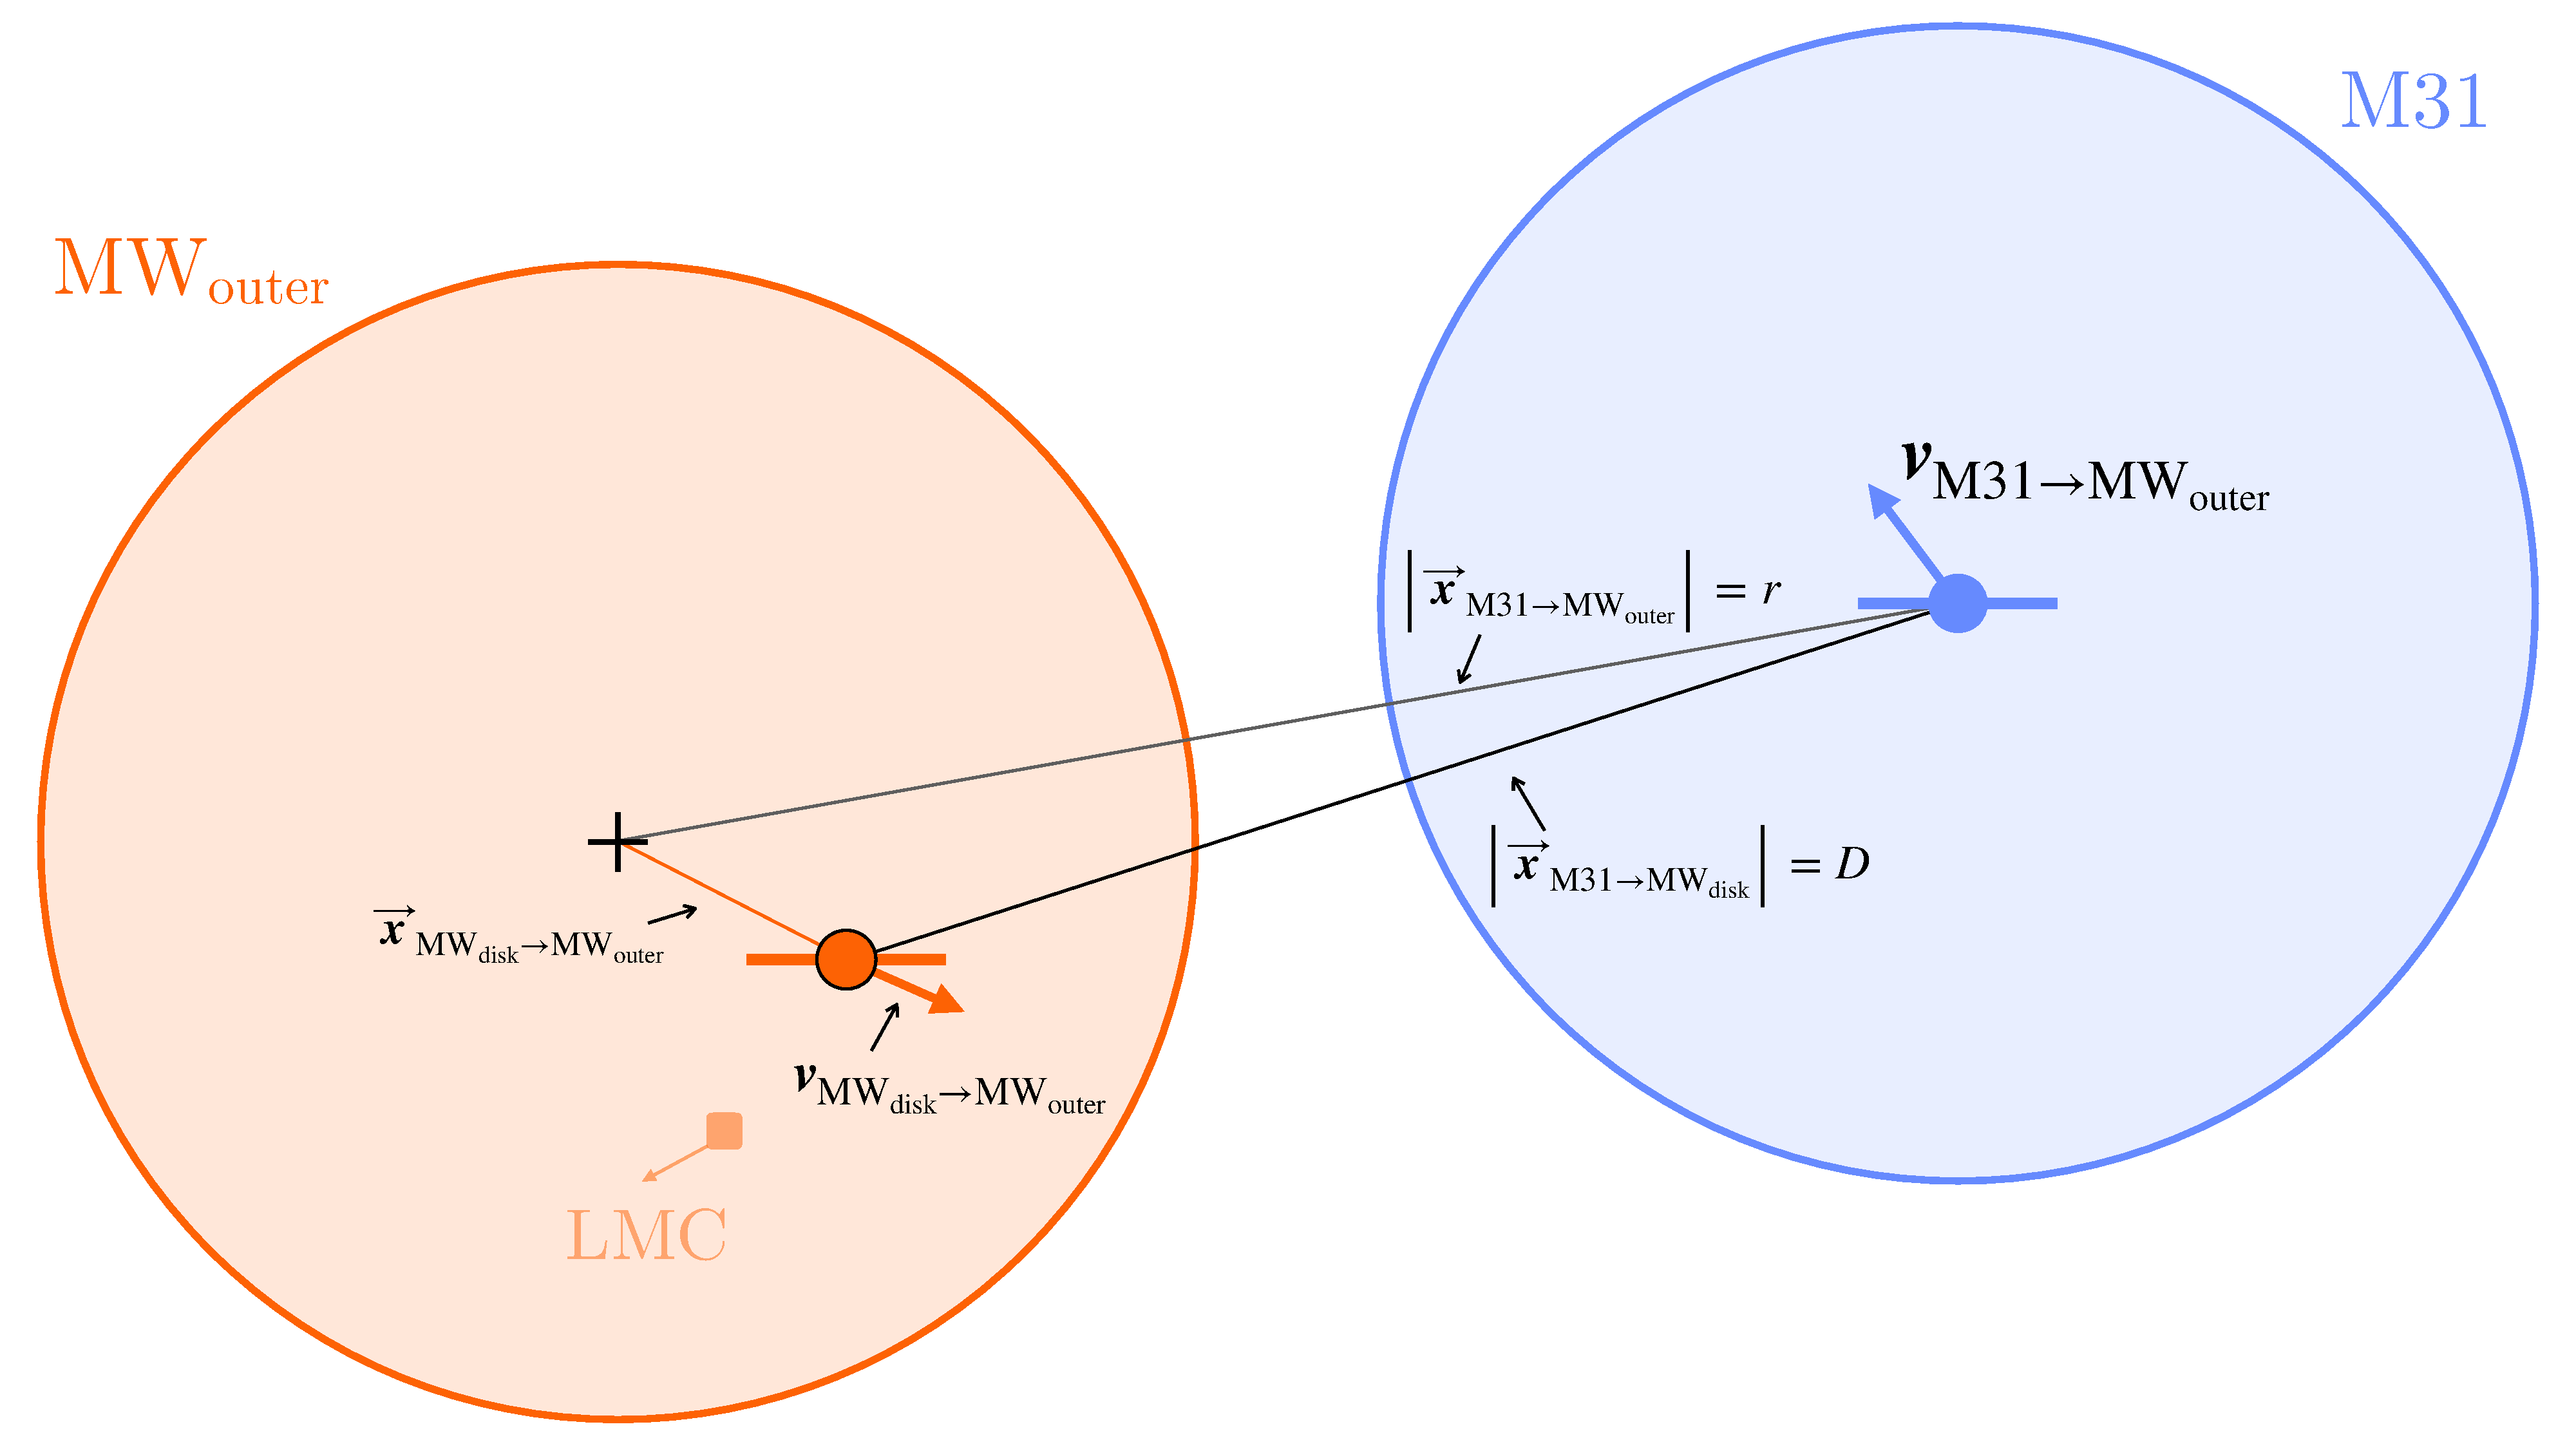
\includegraphics[width=0.8\textwidth]{schematic-filled.pdf}
  \caption{
    Schematic of the MW and M31 system, not to scale. The shaded regions
    represent the halos of both galaxies. Shown are an artistic representation
    of the velocity and position vectors that are relevant in our model,
    including: $\pos{M31}{\mwdisk}$, the distance between the MW disk and the
    M31 disk;
    $\pos{M31}{\mwouter}$, the distance between the centers of both halos;
    $\pos{\mwdisk}{\mwouter}$, the distance between the Galactic center and the
    center of the MW halo (resulting from the reflex motion);
    $\vel{\mwdisk}{\mwouter}$ and $\vel{M31}{\mwouter}$, the velocity of the
    Galactic center with respect to the center of the MW halo, and the measured
    velocity of M31 from the Galactic center, respectively.
    \todo{remove LMC and add note that the travel velocity of the Milky way is from the composite perturbations of many interactions etc.}  }
  \label{fig:schematic}
\end{figure*}


%%%%%%%%%%%%%%%%%%%%%%%%%%%%%%%%%%%
\subsection{Datasets}
\label{sec:datasets}
%%%%%%%%%%%%%%%%%%%%%%%%%%%%%%%%%%%

\todo{Key input into Timing Argument inferences of the Local Group mass are the
present position and velocity of M31 and the age of the universe (used in
Equation~\ref{eq:t}).}
Here we consider three different compilations of data that provide this information to
have as comparisons.
The datasets used in our analysis are summarized in Table~\ref{table:data}. 
\todo{In particular, we consider proper motions from both \textit{HST}~\citep{sohn} and \textit{Gaia}~\citep{Salomon2021} , as well as distance measurements from \cite{vdm2008} and \cite{Li2021}.} 
We have split these measurements into three considered datasets: 
\begin{description}
  \item[vdMG08 Dist. + HST PM] \todo{The first dataset contains the measured proper
  motion of M31 and a collection of other data used to constrain the mass of the
  Local Group via the Timing Argument in~\citet{vdm2012}: This is labeled as
  ``vdMG08 Dist. + HST PM'' in figures below to reflect that the M31 distance
  measurement comes from \citet{vdm2008} and the proper motion comes from HST
  measurements presented in \citet{vdm2012}. For the proper motion components,
  we use the proper motions measured from a combination of satellite kinematics
  and astrometric fields \cite{vdm2012}.}
  \item[Cepheid Dist. + Gaia PM] \todo{As an independent dataset, we also consider a
  compilation of more recent M31 kinematic measurements, including a more
  precise Cepheid-based distance measure to M31 \citep{Li2021} and updated
  proper motions of M31 measured using data from \textit{Gaia} eDR3
  \citep{Salomon2021}. The \textit{Gaia}-based M31 proper motion measurement is
  slightly larger than the HST proper motion of M31, leading to an increased
  implied transverse velocity that leads to a higher inferred Local Group mass
  compared to the more radial orbit implied by the first dataset.}
  \item[Cepheid Dist. + HST PM] \todo{As another comparison, we also use a hybrid
  dataset that uses the Cepheid-based distance measure to M31 and the HST-based
  proper motion measurement \citep{Li2021,vdm2012}.}
\end{description}
See Table~\ref{table:data} for numerical values used in each of these datasets.


\begin{table*}
  \begin{tabular}{lc|c|c}
    \hline\hline
      & \textbf{vdMG08 Dist. + HST PM} & \textbf{Cepheid Dist. + Gaia PM} & \textbf{Cepheid Dist. + HST PM}\\\hline
  $D~[\kpc]$ & $770 \pm 40\reflabel{a}$ &   $761\pm11~\kpc\reflabel{f}$  & $761\pm11\reflabel{f}$\\
  $v_{\rm rad}~[\kms]$ & $-301 \pm 1\reflabel{b}$ & $-301\pm 1\reflabel{b}$ & $-301\pm 1\reflabel{b}$ \\
  $\mu_{\alpha^*}~[\muasyr]$    & $34.30\pm 8.25\reflabel{c}$  & $48.98\pm 10.47\reflabel{g}$ & $34.30\pm 8.25\reflabel{c}$ \\
  $\mu_\delta~[\muasyr]$ & $-20.22 \pm 7.71$\reflabel{c} & $-36.85\pm 8.03\reflabel{g}$ & $-20.22 \pm 7.71$\reflabel{c} \\
  $\bs{v}_\odot$~[\kms]& $(11.1, 251.54, 7.25)\reflabel{d}$ & $(12.9, 245.6, 7.78)\reflabel{h}$ & $(12.9, 245.6, 7.78)$ \reflabel{h}\\
  $t_{\rm peri}~[\Gyr]$ & $13.75\pm 0.11\reflabel{e}$  & $13.801 \pm 0.024$ \reflabel{i} & $13.801 \pm 0.024$ \reflabel{i}\\
  \hline\hline
  \end{tabular}
  \tablerefs{$a.$ \cite{vdm2008},
   $b.$ \cite{Courteau1999},
   $c.$ \cite{vdm2012},\\
   $d.$ \cite{Schonrich2010,McMillan2011},
   $e.$ \cite{Jarosik2011},
   $f.$ \cite{Li2021},
   $g.$ \cite{Salomon2021},\\
   $h.$ \cite{Drimmel2018},
   $i.$ \cite{Planck2018}}
  % \tablenotetext{a}{\cite{vdm2008}}
  % \tablenotetext{b}{\cite{Li2021}}
  \caption{\label{table:data}
  Observational datasets used for comparison throughout analysis and their
  references (vdMG08 is \cite{vdm2008}) Each value is measured for M31 with
  respect to the sun. $D$ is the distance, $v_{\rm rad}$ is the radial velocity,
  $(\mu^*_{\alpha}, \mu_{\delta})$ are proper motions in RA cosdec and Dec, and
  (U$_{\rm pec}$, V$_{\rm pec}$+V$_0$, W$_{\rm pec}$) the solar motion with
  respect to the galactic center. $t_{\rm peri}$ is the time elapsed since the
  last pericenter of the M31 Keplerian orbit, which in this case is the age of
  the Universe.
  }
\end{table*}


%%%%%%%%%%%%%%%%%%%%%%%%%%%%%%%%%%%%
\subsection{Bayesian Inference}
\label{sec:bayes}
%%%%%%%%%%%%%%%%%%%%%%%%%%%%%%%%%%%%

We construct a likelihood function for the observed, Heliocentric position and
velocity of M31 and the time since last pericenter given the four parameters of
the Timing Argument model $(\mlg, a, e, \eta)$, assign prior probability
distribution functions (pdfs) for the parameters, and use these to compute the
posterior pdf over the parameters given the data.
In detail, we first use the four Timing Argument parameters to compute the
present day separation between the MW and M31 and the relative radial and
tangential velocities as defined in Equations~\ref{eq:r}--\ref{eq:vtan}.
These velocity components represent the relative velocity M31 would have as
observed from \todo{the barycenter of the MW--LMC subsystem.}
We then use the measured ``travel velocity'' of \todo{the MW disk
$\vel{\mwouter}{\mwdisk}$} to compute the relative velocity of M31 that would be
\todo{observed from a frame moving with the center of the Milky Way disk (i.e. a
MW Galactocentric frame).}
We finally transform from this Galactocentric frame to a heliocentric
reference frame moving with the solar system barycenter (i.e. ICRS coordinates).
At this final stage, we must introduce an additional nuisance parameter $\alpha$
which represents the orientation of the MW--M31 orbital plane, \kc{ this part sounds confusing to me: }as it intersects
the tangent plane located at the sky position of M31 as viewed from the MW disk
center.
This is necessary because the Kepler equations only provide the magnitude of the
tangential velocity (i.e. Equation~\ref{eq:vtan}), but in order to compute
proper motion components we must also know the exact orientation of the M31
velocity vector.
However, we stress that this position angle has no impact on the fundamental
dynamical parameters and is only used for coordinate transformations.

We specify this model using the \texttt{Python} probabilistic programming
package \texttt{pymc3}~\citep{Salvatier2016} and our adopted prior pdfs are
summarized in Table~\ref{table:priors}.
We use the No-U-Turn Sampler (NUTS) \citep{Homan2014} implemented in
\texttt{pymc3} to generate samples from this posterior pdf, given data from each
of the datasets defined in Table~\ref{table:data}.
We sample over the parameter Local Group mass $\mlg$, \todo{(true) present-day MW--M31}
separation $r$, log eccentricity $\ln\left(1 - e\right)$, eccentric anomaly
$\eta$, and the orbital plane orientation nuisance parameter $\alpha$.
We set the priors as follows:
\begin{itemize}
  \item Mass of the Local Group $\mlg$: we use a broad, truncated normal
  distribution centered on a past measured value of the local group mass.
  \item Present MW--M31 separation $r$: we again use a broad, truncated normal
  distribution centered on past measurements of the distance to M31.
  \item Eccentricity $e$: we assume a uniform prior on eccentricity but sample
  in the transformed parameter $\ln(1-e)$ to improve the acceptance fraction
  when generating posterior samples.
  \item Eccentric anomaly $\eta$: we assume a uniform prior.
  \item Orbital plane orientation $\alpha$: we assume a uniform prior.
\end{itemize}

For each dataset, we run the sampler with 4 chains for 4,000 tuning steps and
40,000 draws.

% \begin{equation}
%   \mathcal{L}(| \boldsymbol{S})
% \end{equation}
% where $\boldsymbol{S} = ($\mlg$, a, e, \eta)$

% TODO: Letters have a 1 table max limit, so we might have to move the prior
% details into the list above. But we could always submit as a short regular
% paper instead of a letter...
\begin{table}
  \centering
  \begin{tabular}{lc}
  \hline\hline
  Prior  & Description \\\hline
  \mlg: $\mathcal{N}_T(4.5,3)\times10^{12}\Msun$ & Mass of the Local Group\\
  %
  $r$: $\mathcal{N}_T(700,100)$kpc & Distance from M31 to $\mwdisk$\\
  %
  $\ln(1-e)$: $\mathcal{U}(-10,0)$ & Eccentricity (close to 1) \\
  %
  $\eta$: $\mathcal{U}(-\pi, \pi)$ & Eccentric anomaly\\
  \multirow{2}{*}{$\alpha$: $\mathcal{U}(-\pi, \pi)$} & Position angle of M31 orbital\\
  & plane from MW disk center\\
  \hline\hline
  \end{tabular}
  \caption{\label{table:priors} A description of our adopted prior probability
  distribution functions over the Timing Argument model parameters.
  Here, $\mathcal{U}(a, b)$ represents a uniform distribution over the domain
  $(a, b)$, and $\mathcal{N}_T(\mu, \sigma)$ represents a truncated Normal
  distribution with mean $\mu$ and standard-deviation $\sigma$.
  We truncate the mass prior pdf to the range $(0.5, 20)\times10^{12} \Msun$ and
  the radius prior pdf to the range $(100, 10^{4})\,\kpc$.
  }
\end{table}


%%%%%%%%%%%%%%%%%%%%%%%%%%%%%%%%%%%
\section{Results: Local group mass estimates}
%%%%%%%%%%%%%%%%%%%%%%%%%%%%%%%%%%%
\label{sec:results}
% \kc{Include the velocity vector of M31 from the halo frame?}

\begin{figure*}[htb]
  \centering
  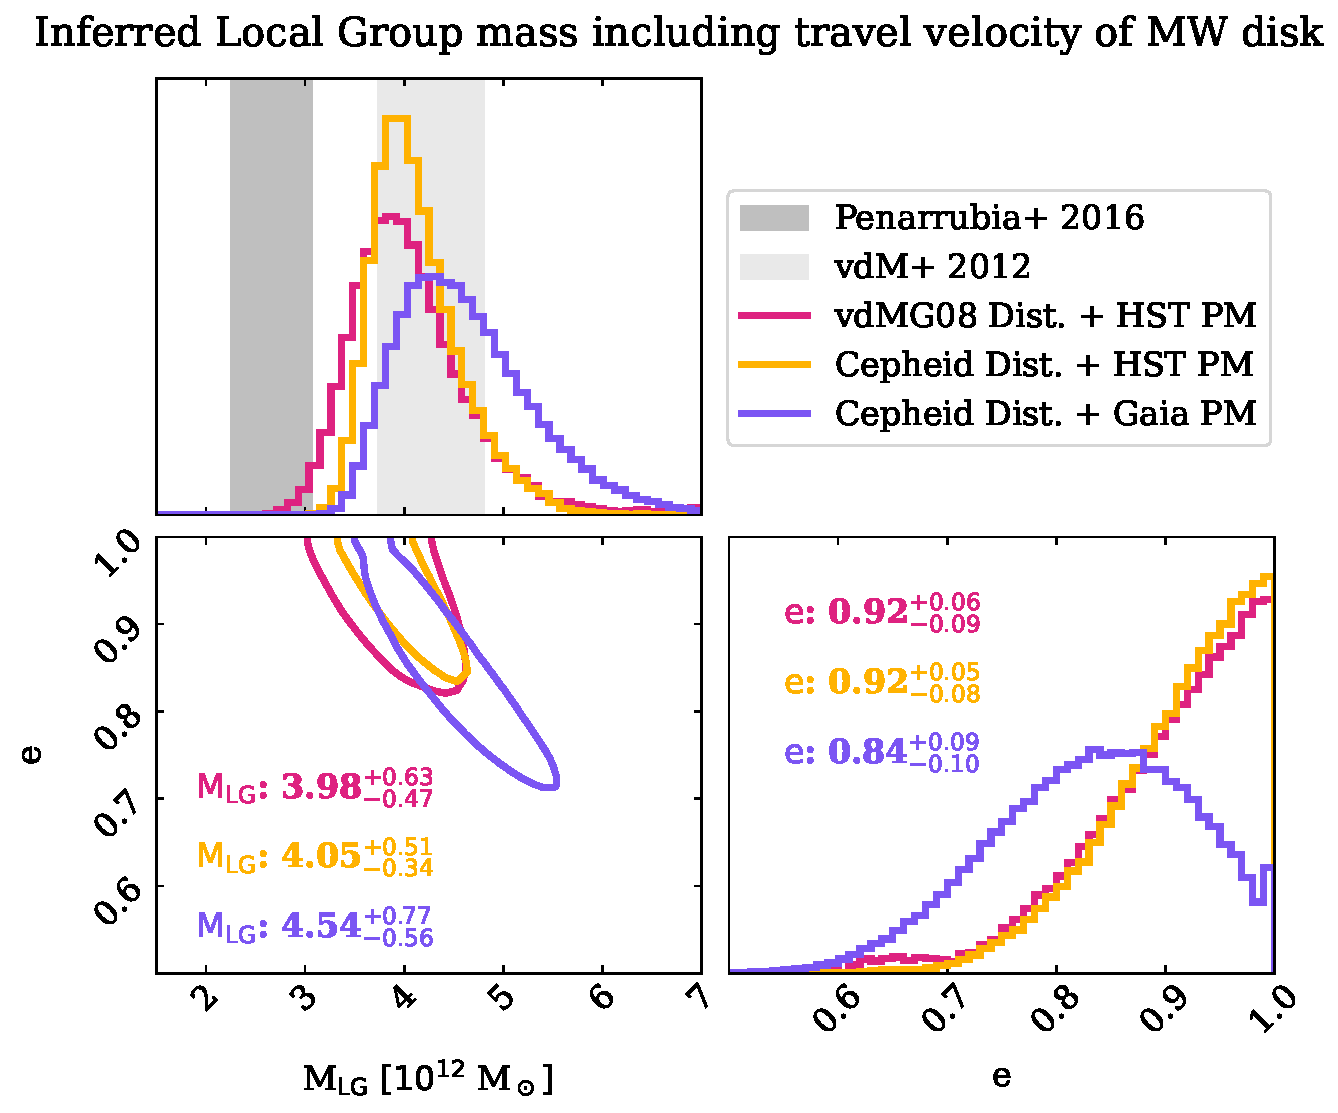
\includegraphics[width=0.8\textwidth,trim=1.3cm 0.8cm 1.3cm 0cm,clip=true]
  {analyze-runs-contour.pdf}
  \caption{\label{fig:contour} 68\% confidence contours of sampled posterior
  distributions with three observational datasets for a subset of our model
  parameters: the total mass of the Local Group (\mlg)
  % , the distance between the Sun and M31 ($r$),
  and the eccentricity of the orbit of M31 about a fixed MW ($e$).
  The more radial orbit implied by the~\cite{vdm2012} \textit{HST} proper
  motions leads to a lower inferred \mlg\ and a higher
  eccentricity, while the larger \textit{Gaia} proper motions of
  ~\cite{Salomon2021} yield a more circular orbit, and thus a lower eccentricity
   and higher mass system.
   \kc{change title of plot}
   }
  % A stationary MW disk is shown in the dotted contours, while our model,
  %which includes the reflex motion of the MW disk, is shown in solid lines.
  % The distributions for the separations are unchanged between models, as our
  % model does not implement a spatial shift to the location of the MW disk.
\end{figure*}

% We use recent measurements of the present-day kinematics of M31 as observed from the solar system, updated measurements of the solar position and motion with respect to the Milky Way center, and a recent measurement of the velocity of the Milky Way disk with respect to the outer stellar halo to measure the mass of the Local Group using observed kinematics of M31.

We use a Bayesian implementation of a Timing Argument model to place constraints
on the mass of the Local Group and the distance between M31 and the Milky Way.
Our model of the Local Group accounts for the \todo{observed reflex motion of 
the Milky Way
disk imparted by the infall of the Magellanic Clouds} and results in new,
less-biased constraints on the mass of the Local Group.
\todo{due to the LMC only? maybe need to be more general about the source?}
  % 4.69$\pm0.71 \times 10^{12}~\Msun$.

We find that our model prefers lower Local Group masses and a lower eccentricity
orbit compared to models that do not include the travel velocity of the \todo{MW disk}.
We also find that the inferred mass is larger and LG orbit is less eccentric
when using the (larger) \gaia\ proper motion of M31.
Figure~\ref{fig:contour} shows a summary of our key results, showing the 68\%
confidence regions from the sampled posterior pdfs of LG mass \mlg\ and
eccentricity $e$.
The upper left panel shows the marginal posterior pdfs over LG mass for each of
the datasets (histogram curves) and with 68\% confidence regions plotted for two
prior LG mass measurements (gray shaded bands).
To summarize: Using the same dataset as used in \citet{vdm2012}
(i.e. dataset \textit{vdMG08 Dist. + HST PM})
, we find a
median posterior LG mass of $\mlg = 3.98 ^{+0.63}_{-0.47}~\Msun$ (where error
bars here report the \todo{68\% confidence interval} around the median), which is
roughly $0.3\times 10^{12}~\Msun$ smaller than reported in \cite{vdm2012}. With
the updated dataset containing \textit{Cepheid Dist + Gaia PM}, we find
$\mlg = 4.54 ^{+0.77}_{-0.56}~\Msun$, while for the combined \textit{Cepheid
Dist. + HST PM} dataset, we find $\mlg = 4.05^{+0.51}_{-0.34}~\Msun$.

For both datasets that use the HST proper motions of M31 
%\citep{vdm2012}
, we
find that the inferred orbital eccentricity is consistent with a radial orbit.
Using the \gaia-based proper motions \citep{Salomon2021} leads to a finite
inferred LG orbital eccentricity of $e\sim 0.85$ and therefore a larger inferred
LG mass.
However, enforcing $e=1$ (i.e. a radial LG orbit) produces very consistent mass
estimates between the datasets considered, implying a LG mass $\mlg = 3.6
\pm 0.3 \times 10^{12}~\Msun$.

% Constraints on the distance to M31 remain roughly unchanged for both datasets, primarily because our model does not introduce a physical displacement of the MW disk, since we assume the motion of the disk over the past XX Myr since the LMC achieved pericenter is negligible compared to the separation between M31 and the MW. Thus, the inclusion of the reflex motion of the disk in our model does not affect constraints on the distance to M31.


\begin{figure}[htb]
    \centering
    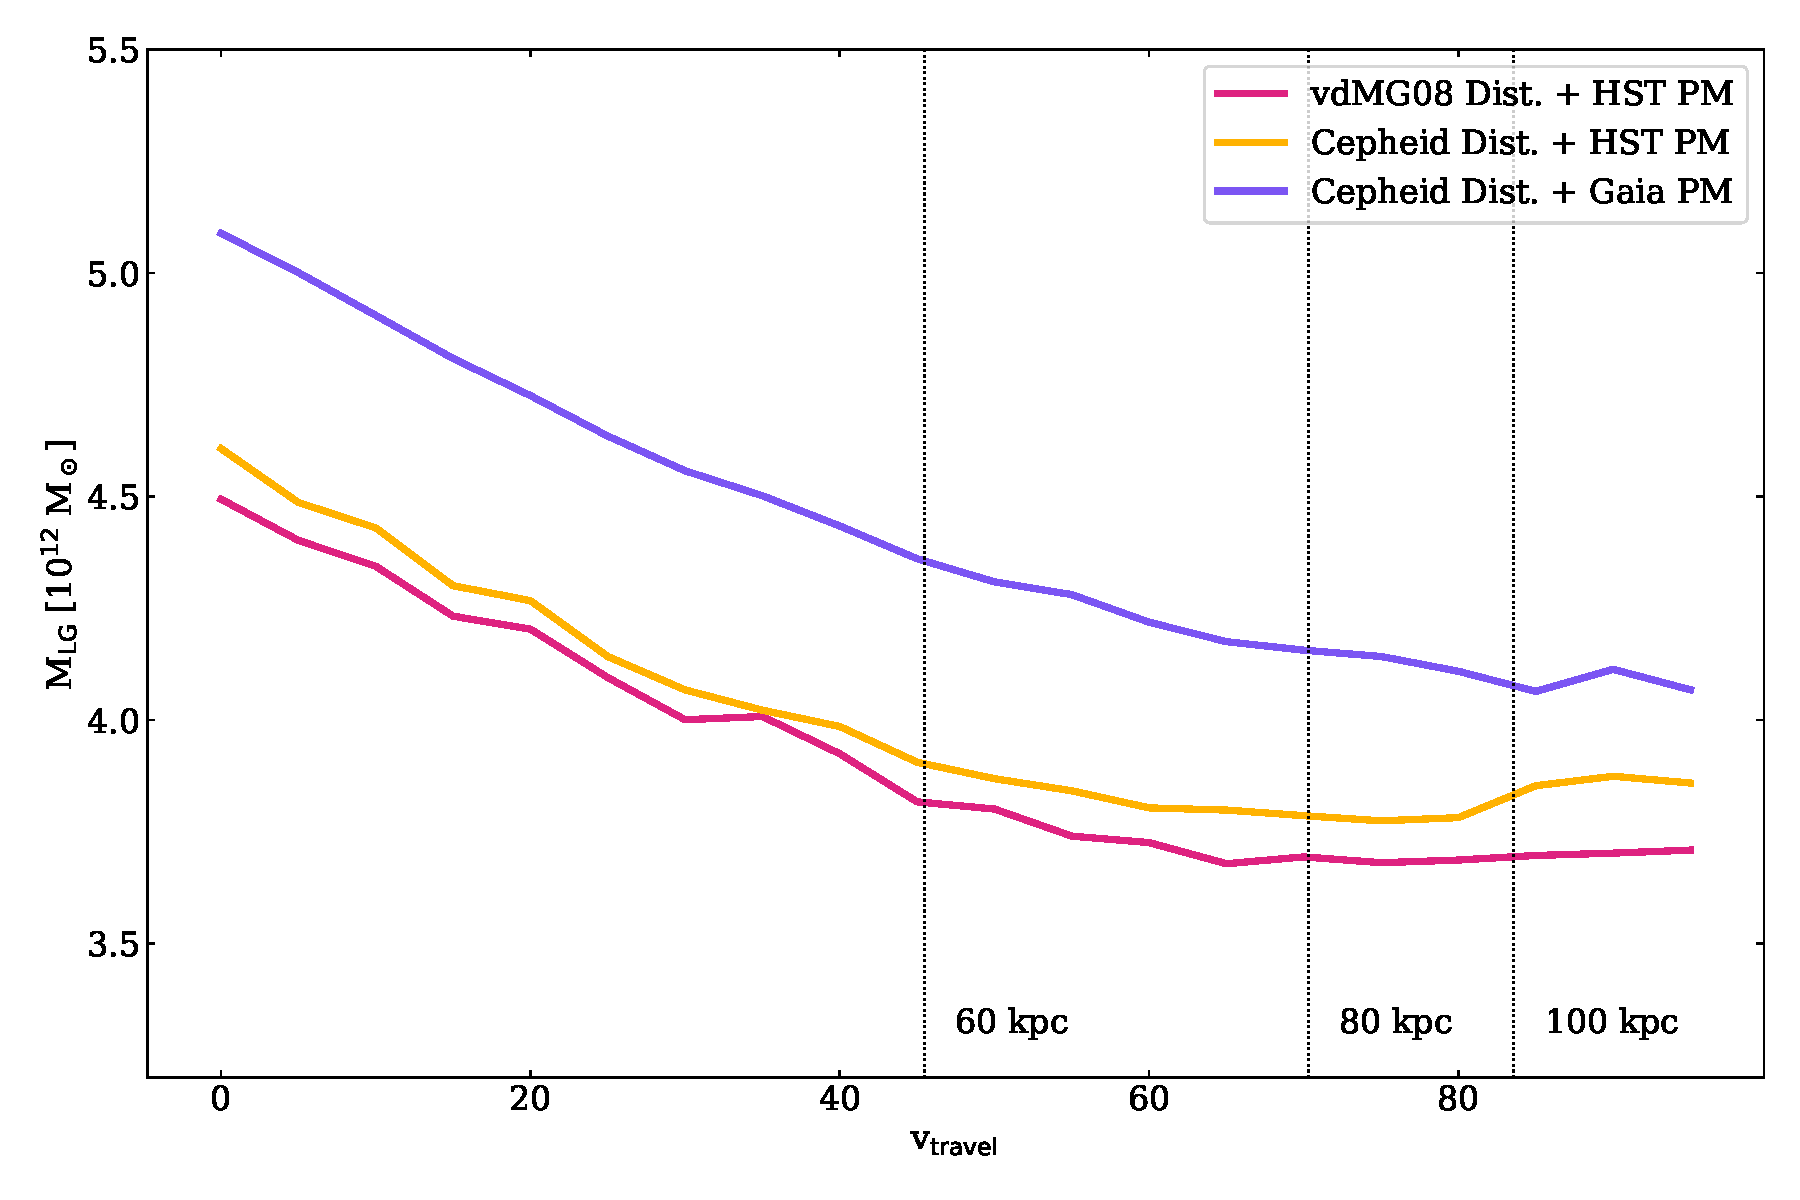
\includegraphics[width=\columnwidth]{analyze-runs-MvsV.pdf}
    \caption{\label{fig:mvsv}
    Mean inferred Local Group mass as a function of travel velocity
    magnitude of the MW disk.
    The larger \textit{Gaia} proper motions (yellow) lead to higher transverse
    motion and thus higher mass than either of the \textit{HST} proper motion
    datasets (pink and purple), though they display the same general trends with increasing travel velocity.
    The vertical lines represent simulated travel velocities for
    stellar tracers at different distances in~\cite{Garavito-Camargo2021b}.
    % The mean Local Group mass corresponding to the observed travel velocity
    % from~\cite{Petersen2021} of 32km/s (triangle points) and the 1-$\sigma$
    % spread on the mass is shown for comparison.
    \textbf{The inclusion of the reflex motion of the MW disk systematically
    lowers the inferred mass of the Local Group} regardless of observational
    dataset.
    \kc{make sense of the leveling off at 70km/s.}
    \todo{make text larger on figure}
    \todo{add large solid line for measured travel velocity}
    \todo{add shaded bands for the estimated vtravel for different mass models of the LMC.}
    }
  \end{figure}

% APW SAYS: I think we can remove this figure and just discuss what it shows in
% the text.
% \begin{figure}[htb]
%     \centering
%     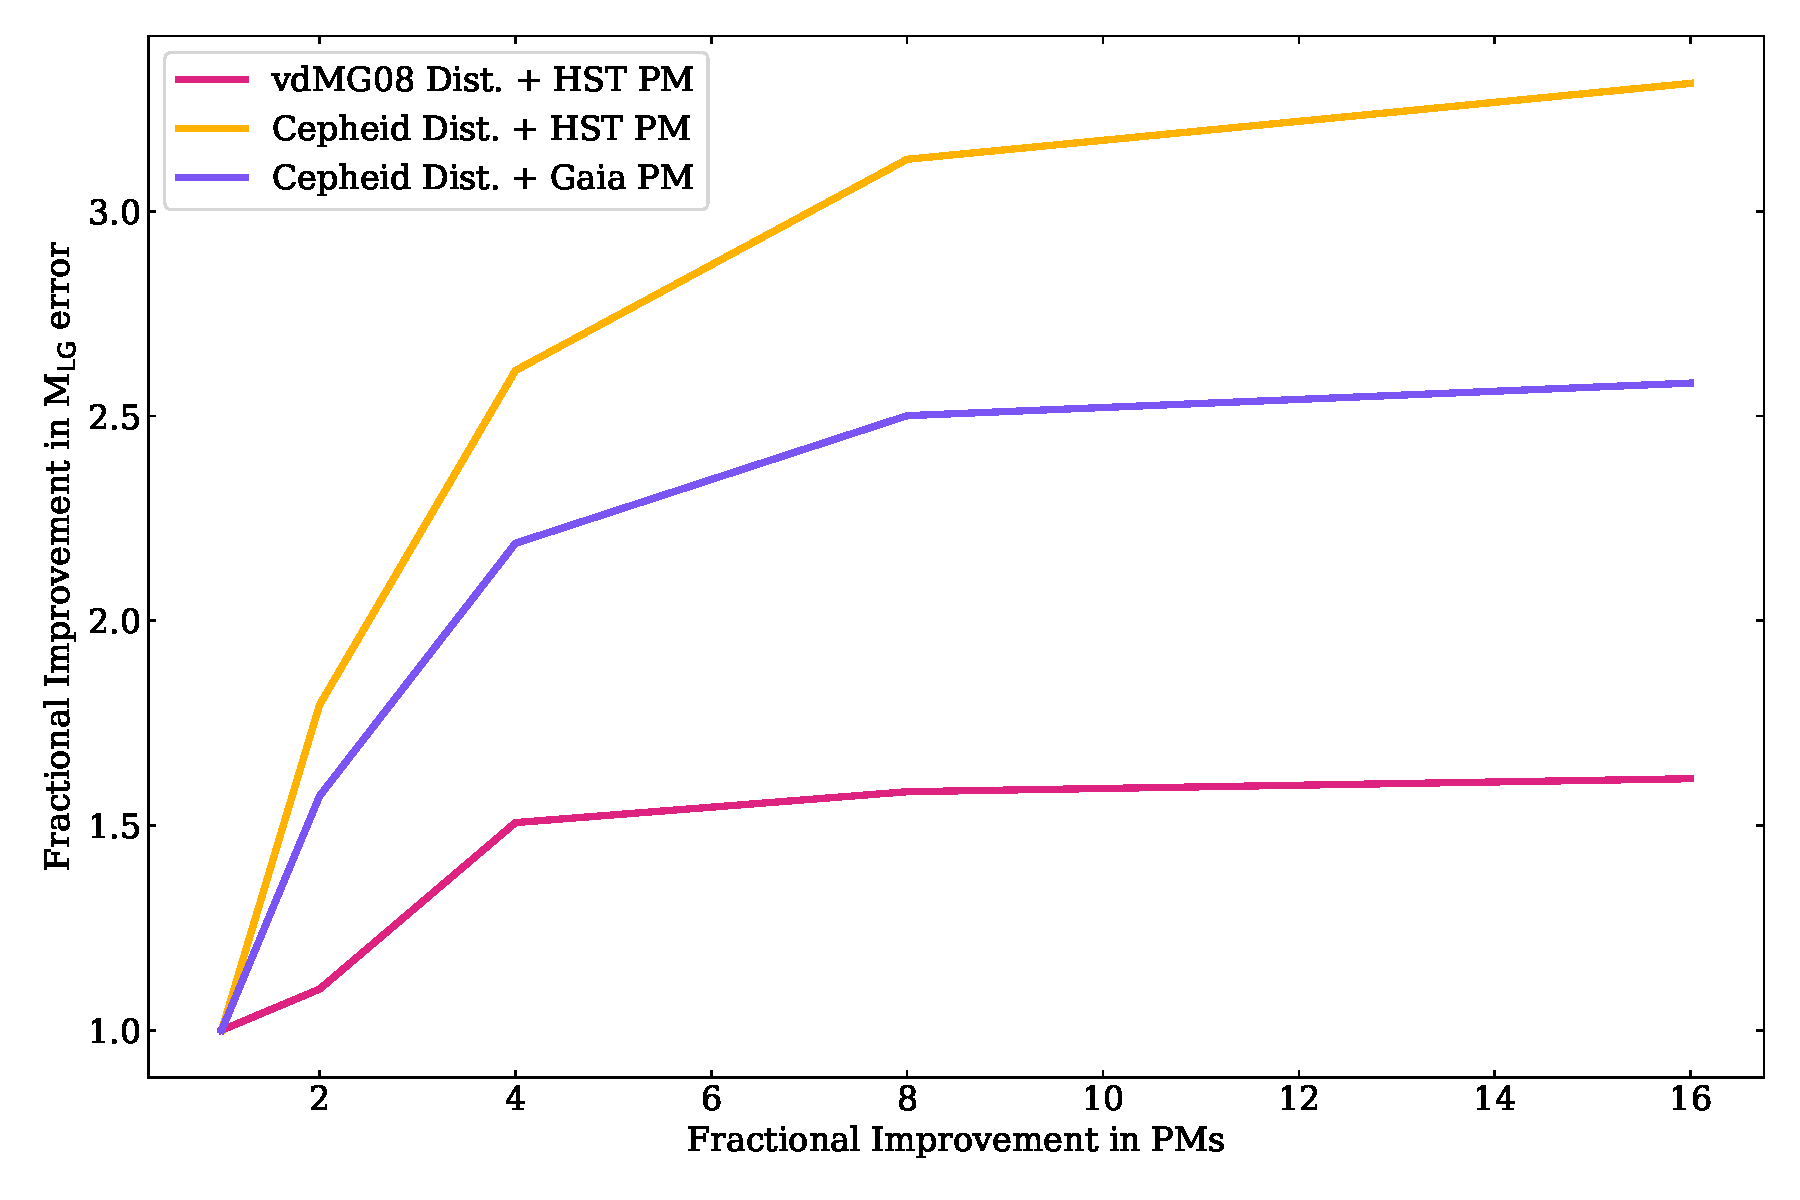
\includegraphics[width=\columnwidth]{analyze-runs-deltaMvsPM.pdf}
%     \caption{\label{fig:mvspm} Improvement in the inferred Local Group mass as a function of fractional improvement in proper motion errors.
%     The standard deviation in the mass decreases with decreasing proper motion
%     error, and in particular, decrease by a factor of $\sim2.5$ for PMs that are
%     4 times smaller than in Dataset 2.
%     \textbf{As future \textit{Gaia} data releases provide improved proper motion errors, constraints on the Local Group mass from the Timing Argument can
%     improve by a factor of $>$2.}
%     }
% \end{figure}

%%%%%%%%%%%%%%%%%%%%%%%%%%%%%%%%%%%
\section{Discussion}
\label{sec:discussion}
%%%%%%%%%%%%%%%%%%%%%%%%%%%%%%%%%%%

\subsection{Comparing recent measurements of the Local Group mass}

\apw{Add a paragraph comparing our measurements to other values (e.g., summarize aspects of your Table 3)}

Suggested outline:
- There are two ways of measuring LG mass: go after it directly with LV dynamics / Timing Argument, or measure MW/M31 separately and add the masses

- Historically, LG dynamics-inferred masses are larger than adding MW+M31 masses: recap rough numbers from your Table 3 (LG dynamics masses have been upwards of $4\times 10^{12}$, adding independent mass measures closer to 2--2.5)

- One exception is the Penarrubia2016 method, ... (use sentences from paragraph below to describe)

- Our value is still larger than most added MW+M31 values (except Cosmo sims), but brings it closer to MW+M31

- Not surprising there is some discrepancy because MW/M31 total mass estimates do not measure full extent of DM distribution and have to extrapolate - there are large uncertainties

- Other TA models and what their differences have been. Namely, here compare Benisty and the fact that they use: 
model-dependent transverse velocity corrections
Gaia PMs only


~\cite{Penarrubia2016} finds a Local Group mass of ($\sim2.64\pm0.4\times
10^{12}~\Msun$) which is significantly lower than our expectations, although this
constraint combines the observed kinematics of 35 Local Volume galaxies in
addition to the dynamics of the M31--MW system.
Each of the Local Volume Galaxies is fit to a radial Keplerian orbital model.
However, inclusion of any transverse motion will increase the inferred total
mass of the system, so it is likely the assumption of radial orbits leads to
an underestimate of the mass of the Local Group with LV galaxies only.
Including the dynamics of the M31--MW system increased their recovered
total mass by $0.6\times10^{12}~\Msun$.

\kc{The \cite{Benisty2022} paper reports a Local Group TA mass of
$5.6^{+1.6}_{-1.2}\times10^{12}\Msun$ after correcting for the reflex motion
of the MW induced by the LMC, which is roughly 25\% larger than our findings.
The discrepancy is likely due to differences in correcting for the reflex motion
of the MW disk.
They find that cosmic bias lowers the TA mass by an additional 40\%.
The large errorbars are likely due to uncertainties in the orbital modelling of
M31 about the combined MW--LMC system.}



\subsection{Correction for ``Cosmic Bias''}

Given the simplicity of the Timing Argument dynamical model --- in particular,
the assumption that the MW and M31 are point masses with constant masses --- it
is reasonable to wonder whether this methodology provides unbiased estimates of
the true LG mass.
An early study of a dark-matter-only cosmological simulation found that the
Timing Argument applied to pairs of galaxies did provide unbiased estimates of
the sum of masses of the pairs \citep{LiWhite2008}.
However, more recently it was found that conditioning on LG-analogs with similar
radial and tangential velocities to the MW and M31 leads to slightly biased
(overestimated) inferred total masses of those systems \citep{Gonzalez2014,
Hartl2021}.
In this work, we do not attempt to ``correct'' our inferred LG masses for this
cosmic bias effect, because it is unclear whether cosmological simulations
accurately reproduce the detailed properties of LG systems.
Accounting for this effect would likely lower our LG mass measurements.


\subsection{Inclusion of \todo{Milky Way disk reflex motion in dynamics of the Local Group}}

As shown in our results above, including the \todo{reflex motion of the Milky Way disk
results in measurable differences in the estimated mass of the Local Group
through the Timing argument.
Ignoring this motion at its currently measured travel velocity}\footnote{Defined
as \todo{$\vel{\mwouter}{\mwdisk}$ above.} magnitude of $v_\textrm{travel} = 32~\kms$}
\citep{Petersen2021} leads to LG masses that are overestimated by $\sim30\%$.
However, the direction and magnitude of travel velocity is directly tied to the
inferred mass of the Local Group.
As it is currently measured, the (mean) direction of $\vel{\mwouter}{\mwdisk}$
is just $\sim$$60^\circ$ from the sky position of M31, meaning that the travel
velocity impacts the conversion of both M31's observed proper motion and radial
velocity from a Heliocentric reference frame to the ``outer halo'' reference
frame used above.
At fixed magnitude, if the true apex of the travel velocity motion is closer
(farther) to M31's sky position, it would primarily affect the radial velocity
(proper motions).

% Thus, the observed radial velocity of M31 will be higher than for an unperturbed MW halo. Since $-v_{rad}\propto M^{1/2}$ for an infalling system, a smaller (but still negative) radial velocity will yield a lower Local Group mass.

% The eccentricity decreases significantly for Dataset 2 compared to Dataset 1, due to the larger measured proper motions of Dataset 2.  Additionally, a smaller radial velocity corresponds to a lower eccentricity for a fixed mass and distance, which can be seen in the bottom right panel of~\ref{fig:contour}.

% bit about the stellar halo tracers and different distances etc
There is reason to believe that the recently measured MW disk travel velocity
could be a lower bound on the true value, which could be up to a factor of
$\sim$2--3 higher than the currently measured value.
Using an idealized simulation of an equilibrium dark matter halo that has a
recent merger with an LMC-like halo, \cite{Garavito-Camargo2021b} showed that
stellar halo tracers at different distances from the MW disk center may result
in different measured travel velocities.
\todo{while this simulation does not span previous mergers in the MW's history, it gives a good first order approximation of what we may expect}
% , and it is possible that the current measurement on $v_{travel}$ of 32km/s are just a lower bound on the actual reflex motion of the disk.
At fixed apex direction, a larger travel velocity would correspond to a lower
inferred LG mass.
Figure~\ref{fig:mvsv} shows the effect of increasing the measured travel
velocity magnitude and its impact on the inferred mass of the Local Group for
each of the datasets used in this work (see Section~\ref{sec:datasets}).
The vertical lines in this figure show the travel velocities that are predicted
for three tracer distances in simulations from~\cite{Garavito-Camargo2021b} \todo{If adding shaded bands to the plot, going to have to explain those here}.
% \kc{why does the mass level off after 80kpc / 70km/s? }
Thus, future measurements of the travel velocity of the disk that use tracers at
larger distance around the MW stellar halo will likely lead to a lower inferred
Local Group mass.

\subsection{Improved \mlg\ constraints from future observations}

The biggest source of uncertainty in our empirically inferred LG mass $\mlg$ currently comes
from the proper motion measurements, which currently have signal-to-noise ratios
of just 3--4.
Future data releases from the \gaia\ Mission \citep{GaiaOverview2016} will lead
to more precise mean proper motions of M31 and thus more precise Timing Argument
constraints on the LG mass.
For example, between \gaia\ EDR3 and the end of the extended (10 year) mission,
the expected individual-source proper motion precision improvement for a $G=20$
source (i.e. an upper giant-branch star in M31) is a factor of $\sim$6.
Na\"ively scaling the proper motion uncertainties of M31 as measured with \gaia\
\citep{Salomon2021} by a factor of 6 leads to a $\sim2\times$ improvement in the
$\mlg$ precision.
Of course, the true improvement of the mean M31 proper motion with improved
individual source kinematics could be even better than linear because more
sources will be detected and usable in the measurement.


\subsection{The M31--M33 system\todo{change}}
\todo{short sentence about the M31 subsystem and how we absolutely do not attempt to add in a travel velocity.}
While M31 has a massive satellite (M33) of comparable mass ratio to the
MCs--Milky Way system, we do not expect there to be a significant reflex
velocity of M31's disk relative to its equivalent outer halo reference frame:
Recent work predicts that M33 is likely on first infall into the M31 halo and
has a much larger orbital pericenter than the MCs \citep[e.g.,][]{Patel2017a}.
On the other hand, M31 has likely experienced other significant mergers, as
evidenced by the double nucleus and Giant Southern Stream
\citep[e.g.][]{Ibata:2001, Font:2006}, but these were likely lower mass-ratio
mergers \citep[e.g.][]{Gilbert:2019, Milo:2022} and thus will have less of an
impact on the bulk motion of the M31 disk.
\todo{Given current knowledge of the M31 system and uncertainties in the orbital
histories of its most massive satellites, here we neglect the (likely
subdominant) reflex motion of the M31 disk.}
\todo{However, a measurement or upper limit on the M31 disk travel velocity would
enable further unbiased constraints on the Local Group mass.}

%%%%%%%%%%%%%%%%%%%%%%%%%%%%%%%%%%%
\section{Summary and Conclusions}
%%%%%%%%%%%%%%%%%%%%%%%%%%%%%%%%%%%
\label{sec:summary}
\todo{check numbers in this paragraph}
In this Letter, we use the Timing Argument to constrain the mass of the Local
Group by modeling the relative dynamics of the Milky Way (MW) and M31,
accounting for the recently-measured travel velocity of the MW disk with respect
to the outer stellar halo of the Galaxy.
We show that accounting for the travel velocity of the MW disk lowers the
inferred Local Group mass from the Timing Argument when compared to a prior
result using the same compilation of M31 kinematic measurements, finding $\mlg =
3.98\times 10^{12}~\Msun$.
Using more recent distance and proper motion measurements of M31 we find that
the orbit of the Local Group galaxies is less radial than previously found,
leading to a slightly higher inferred Local Group mass $\mlg = 4.54\times10^{12}~\Msun$.

\todo{clean up or rewrite a big-picture concluding paragraph?}
Our findings of a high mass Local Group are consistent with findings that the
mass of M31 is XXbig and the MW is $1-1.5\times10^{12}~\Msun$~\citep{??}.
However, this high group mass also has cosmological implications.
A high Local Group mass could also be consistent with tk that propose that M31
has undergone recent (XX Gyrs) major? accretion events with other massive
subhalos, resulting in morphological features like the Giant Southern Stream and
XX (what are other M31 things that indicate recent interactions? Do we think
much about M32? )

% \subsection{Cosmological implications}
\begin{table*}
  \centering
  \begin{tabular}{clc|c}
    \hline\hline
    Mass & Method & Result ($ 10^{12}~\Msun$ ) & Citation \\\hline
    \multirow{7}{*}{\mlg}  &{LV Galaxies + Timing Argument} & {2.64$\pm0.4$} & \cite{Penarrubia2016} \\
    &{Timing only} & {4.27$\pm$0.45} & \cite{vdm2012} \\
    &{Timing (3D + cosmic bias and scatter)} & {4.93$\pm$1.63} & \cite{vdm2012} \\
    &Timing (radial + cosmo sim calibration)  & $5.27$& \cite{LiWhite2008} \\
    &Timing & $3.6$ & \cite{Lynden-Bell:1981} \\
    & Cosmo Sims & 4.4$^{+2.4}_{-1.5}$ & \cite{Zhai2020}\\
    & LG Dynamics &$2.5\pm0.4$ & \cite{Diaz2014}\\
    %  &  &  \\
    \hline
    \multirow{3}{*}{\mmto}& Kinematics of M31 Sats & $1.4 \pm 0.4$ ($<$300 kpc) & \cite{Watkins2010}\\
    & Cosmo Sims & 2.5$^{+1.3}_{-1.1}$ & \cite{Zhai2020}\\
    & LG Dynamics &$1.7\pm0.3$ & \cite{Diaz2014}\\
    \hline
    \multirow{4}{*}{\mmw}&  Kinematics of LG sats & $1.4 \pm 0.3$ ($<$300 kpc) & \cite{Watkins2010}\\
    & Cosmo Sims & 1.5$^{+1.4}_{-0.7}$ & \cite{Zhai2020} \\
    & LG Dynamics &$0.8\pm0.5$ & \cite{Diaz2014}\\
    & MW Sats & $0.96^{+0.29}_{-0.28}$ & \cite{Patel2017}\\
  \hline\hline
  \end{tabular}
  \caption{\label{table:masses}Can remove this, this is just to keep me sane}
\end{table*}

% Previous uses of the Timing Argument have placed constraints on the mass of the Local Group

% By including reflex motion, we move in the direction of the expected summed masses of the Milky Way and M31 which is good.

% How does the mass that we found compare to mass estimates from other means?
% - like hubble flow constraints, previous timing argument, previous MW--M31 measurements, etc.



% If our mass is higher, what does that mean?
% If our mass is lower, what does that mean?
% What does this high mass mean to the Local Group? What about to the
% constituents?

% What is context for mergers and M31 and why they might be
% related to the Local Group mass?


\begin{acknowledgements}

This project was started at the Big Apple Dynamics School (BADS) hosted by the
Flatiron Institute July--August 2021.
We greatly benefitted from discussions with the other students who attended the
BADS, and received helpful input from:
Kathryn Johnston (Columbia),
\todo{Who else?}.
This work made use of the
\texttt{PyGaia}\footnote{https://github.com/agabrown/PyGaia} package: We
acknowledge the Gaia Project Scientist Support Team and the Gaia Data Processing
and Analysis Consortium (DPAC) for their work on this software tool.
This research made use of Astropy,\footnote{http://www.astropy.org} a
community-developed core Python package for Astronomy \citep{astropy:2013,
astropy:2018}.
\end{acknowledgements}

\software{
    Arviz \citep{arviz},
    Astropy \citep{astropy:2013, astropy:2018},
    gala \citep{gala},
    IPython \citep{ipython},
    matplotlib \citep{matplotlib},
    numpy \citep{numpy},
    pymc3 \citep{Salvatier2016},
    scipy \citep{scipy}
}

\appendix
Currently, appendix only includes the corner plots for all of the 5 model parameters for each of the three datasets.
\begin{figure*}[htb]
  \centering
  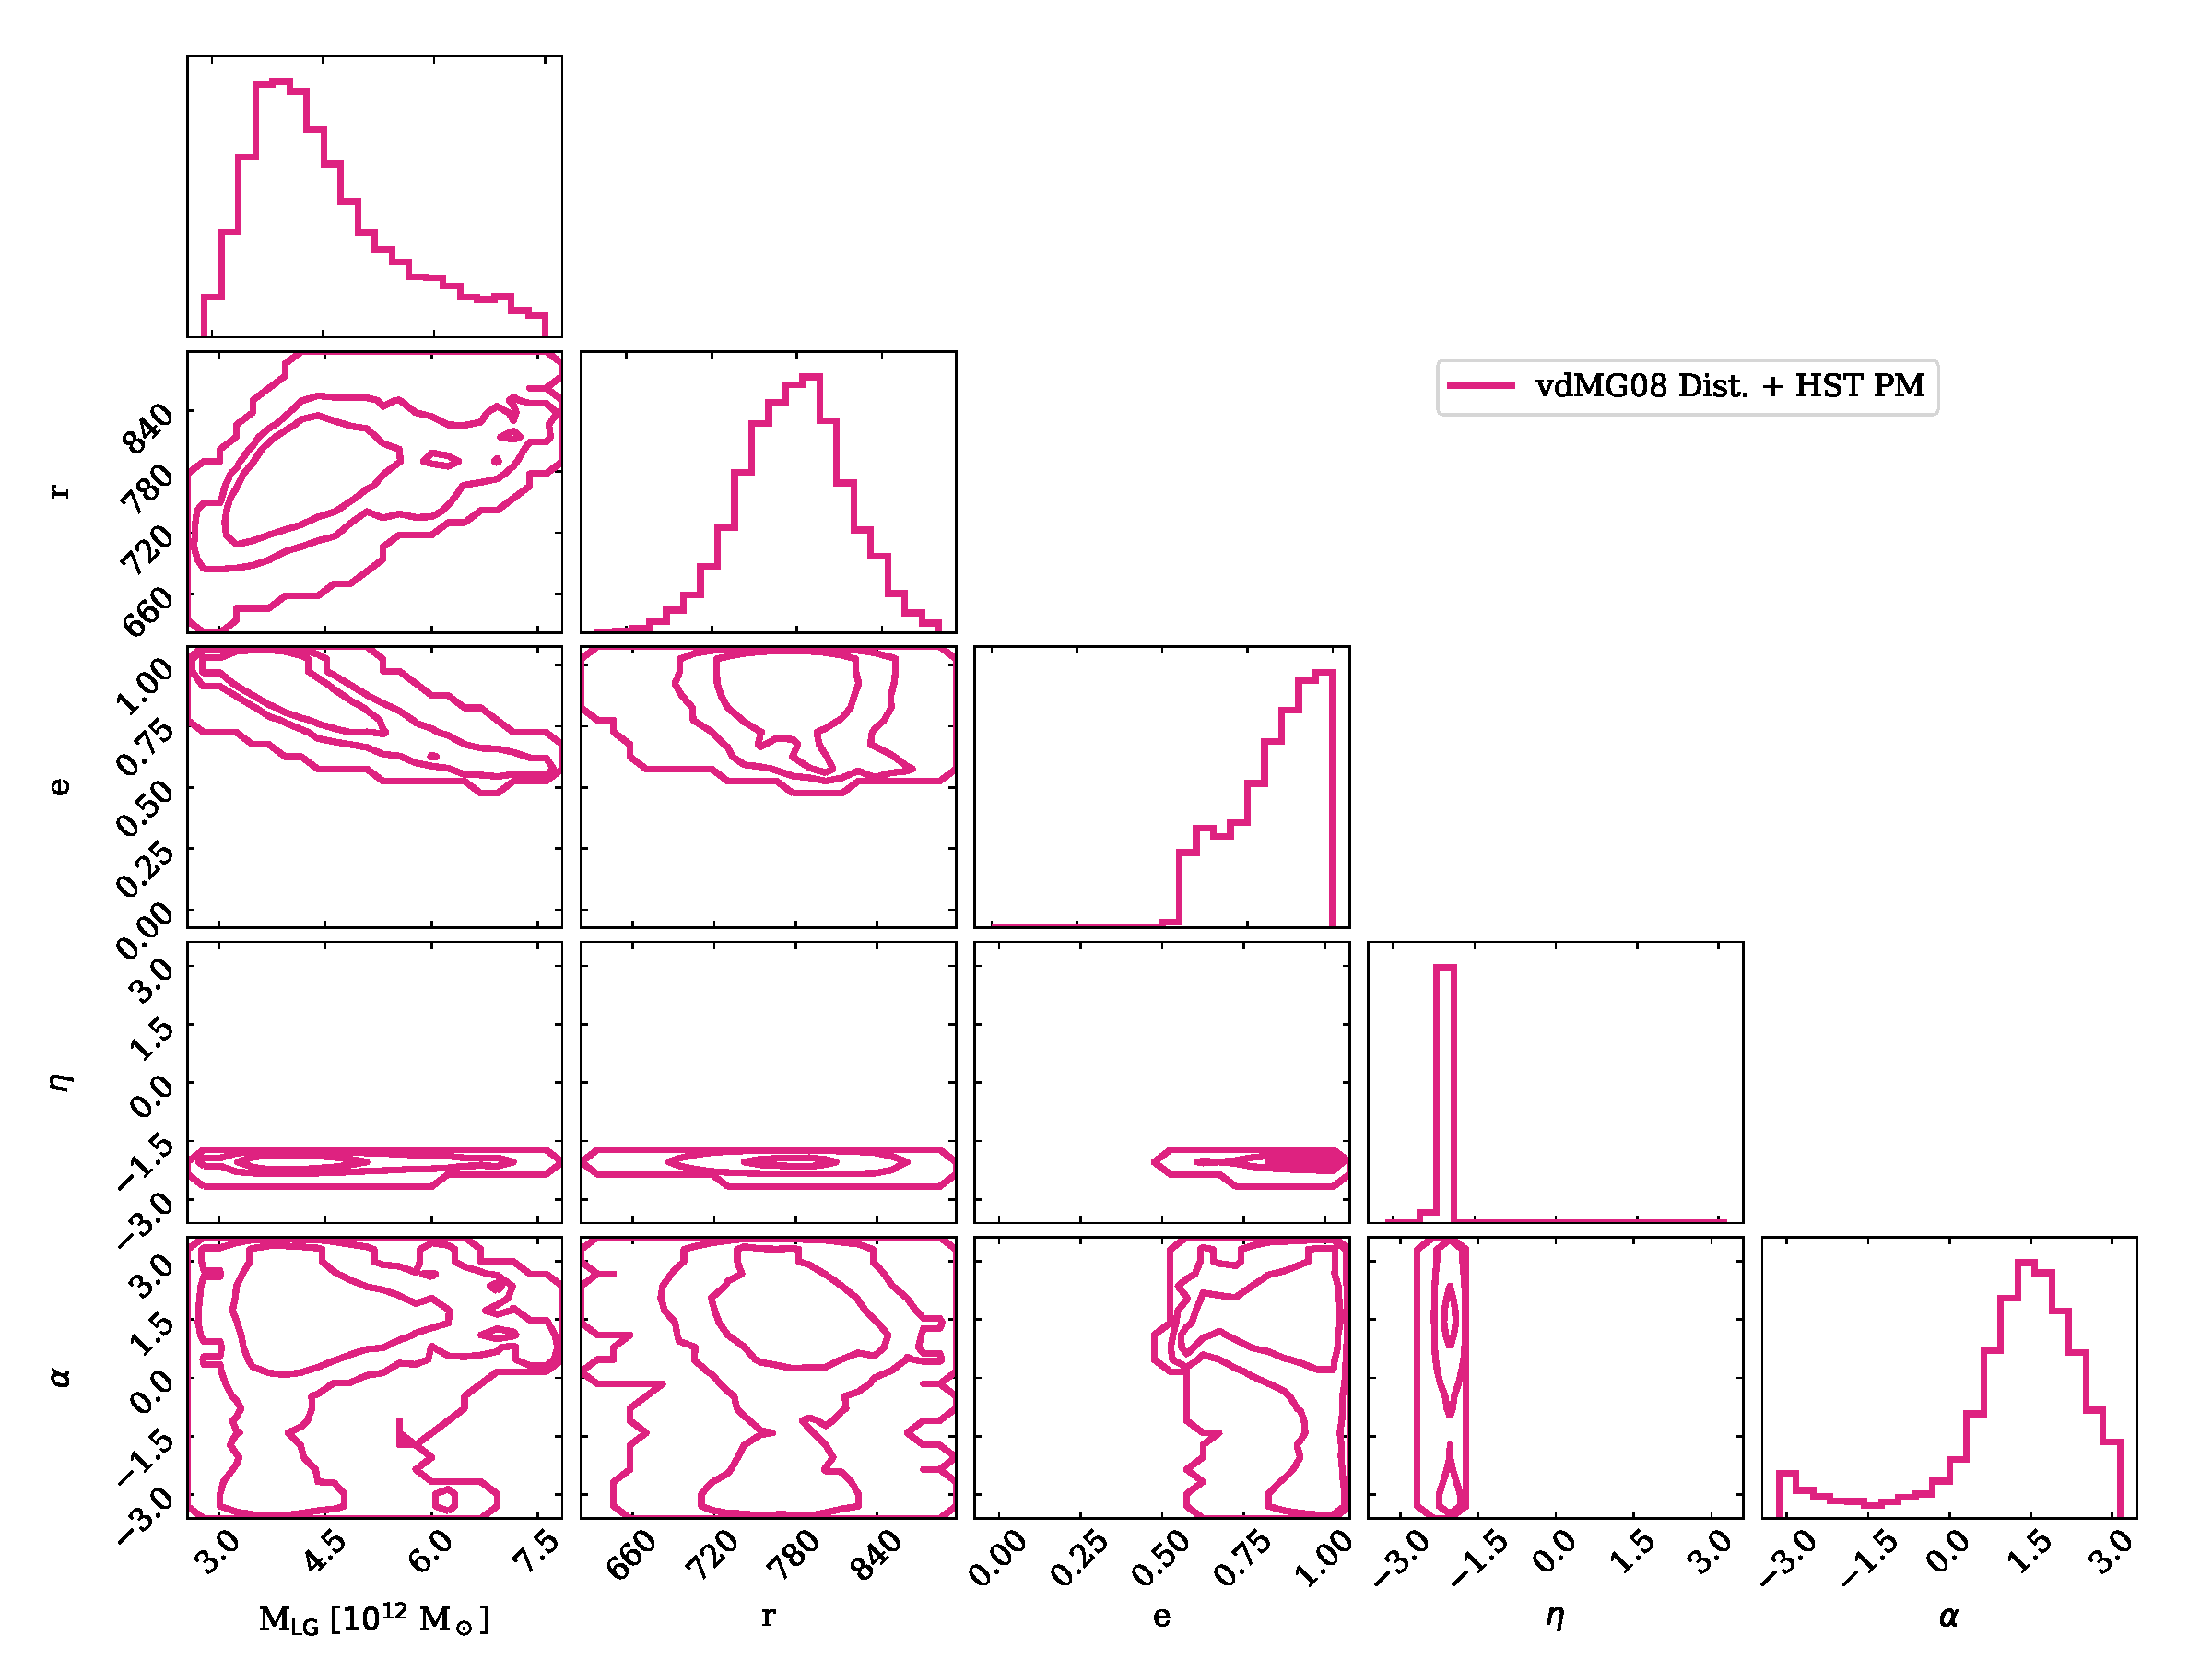
\includegraphics[width=0.8\columnwidth]{analyze-runs-all-vdm2012.pdf}
  \caption{\label{fig:contour-vdm}
  68\% and 95\% confidence contours of sampled posterior distributions for all
  model parameters for the vdMG08 (how to make link to citation?) distance
  measurement $770\pm 40 \rm kpc$ and proper motions from \textit{HST}.
  }
\end{figure*}

\begin{figure}[htb]
  \centering
  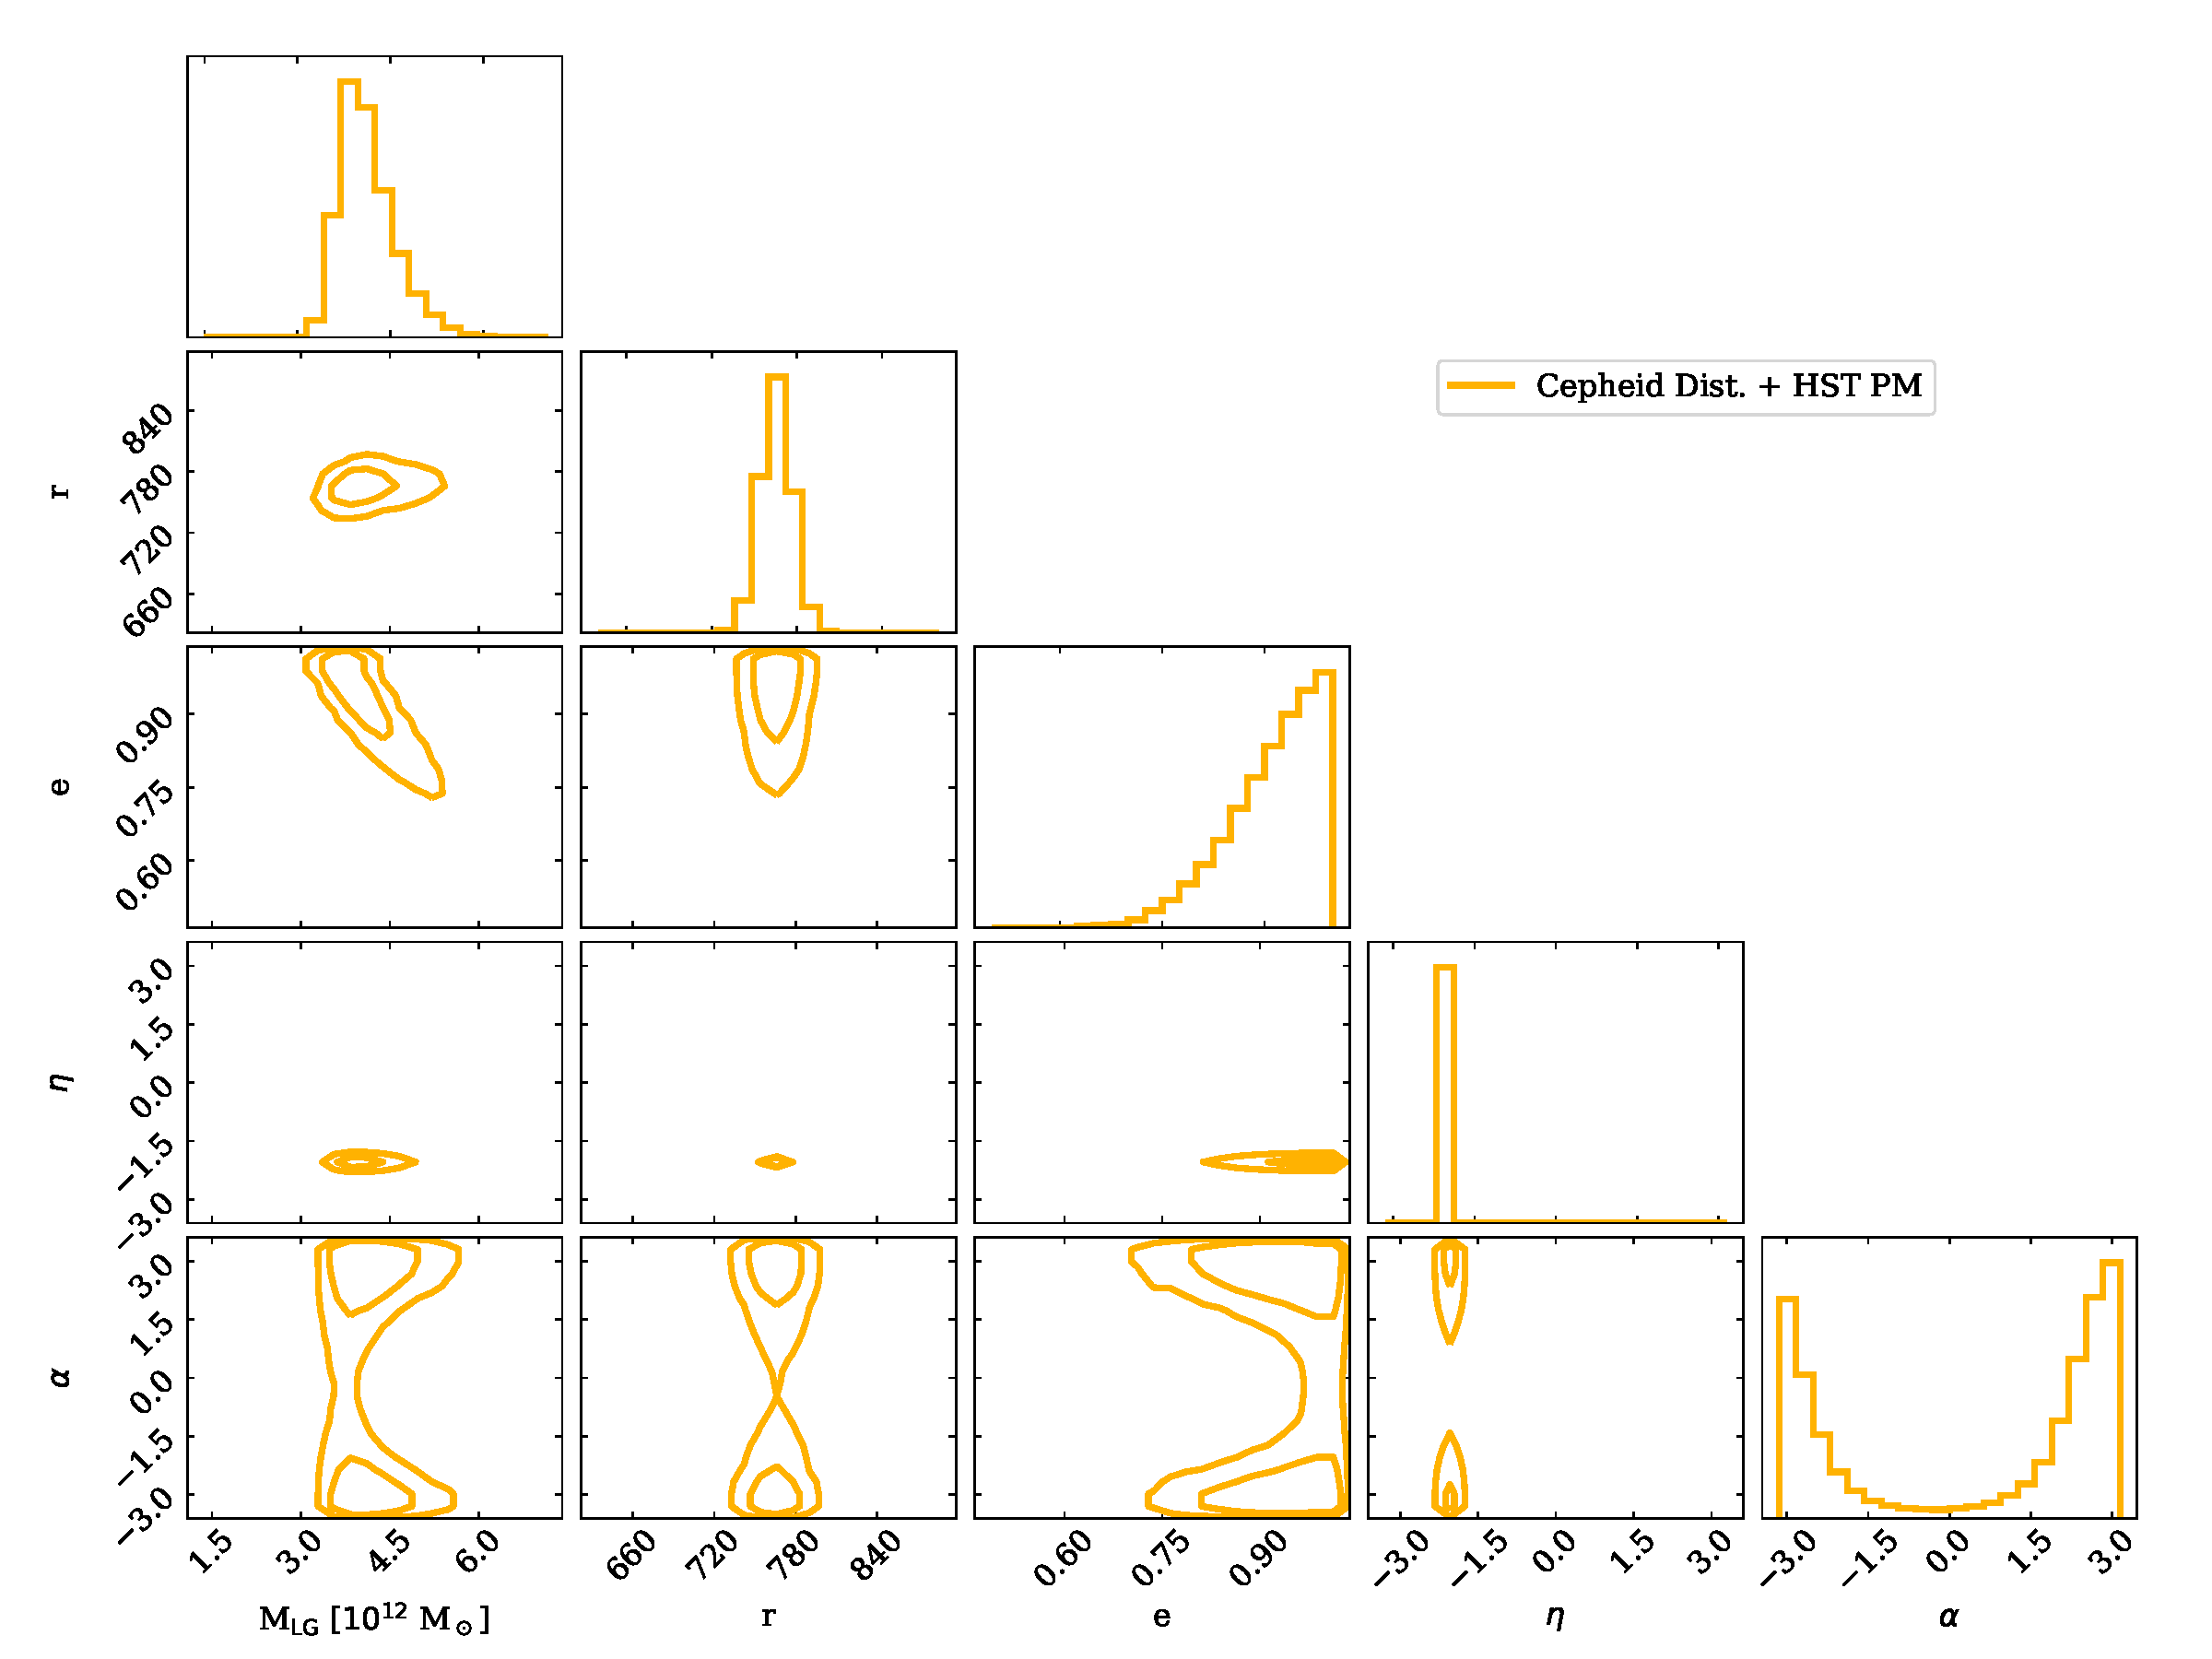
\includegraphics[width=0.8\columnwidth]{analyze-runs-all-Dataset3.pdf}
  \caption{\label{fig:contour-dataset3}
    68\% and 95\% confidence contours of sampled posterior distributions for all
    model parameters for the vdMG08 (how to make link to citation?) distance
    measurement $770\rm kpc$ and proper motions from \textit{HST}.
  }
\end{figure}

\begin{figure*}[htb]
  \centering
  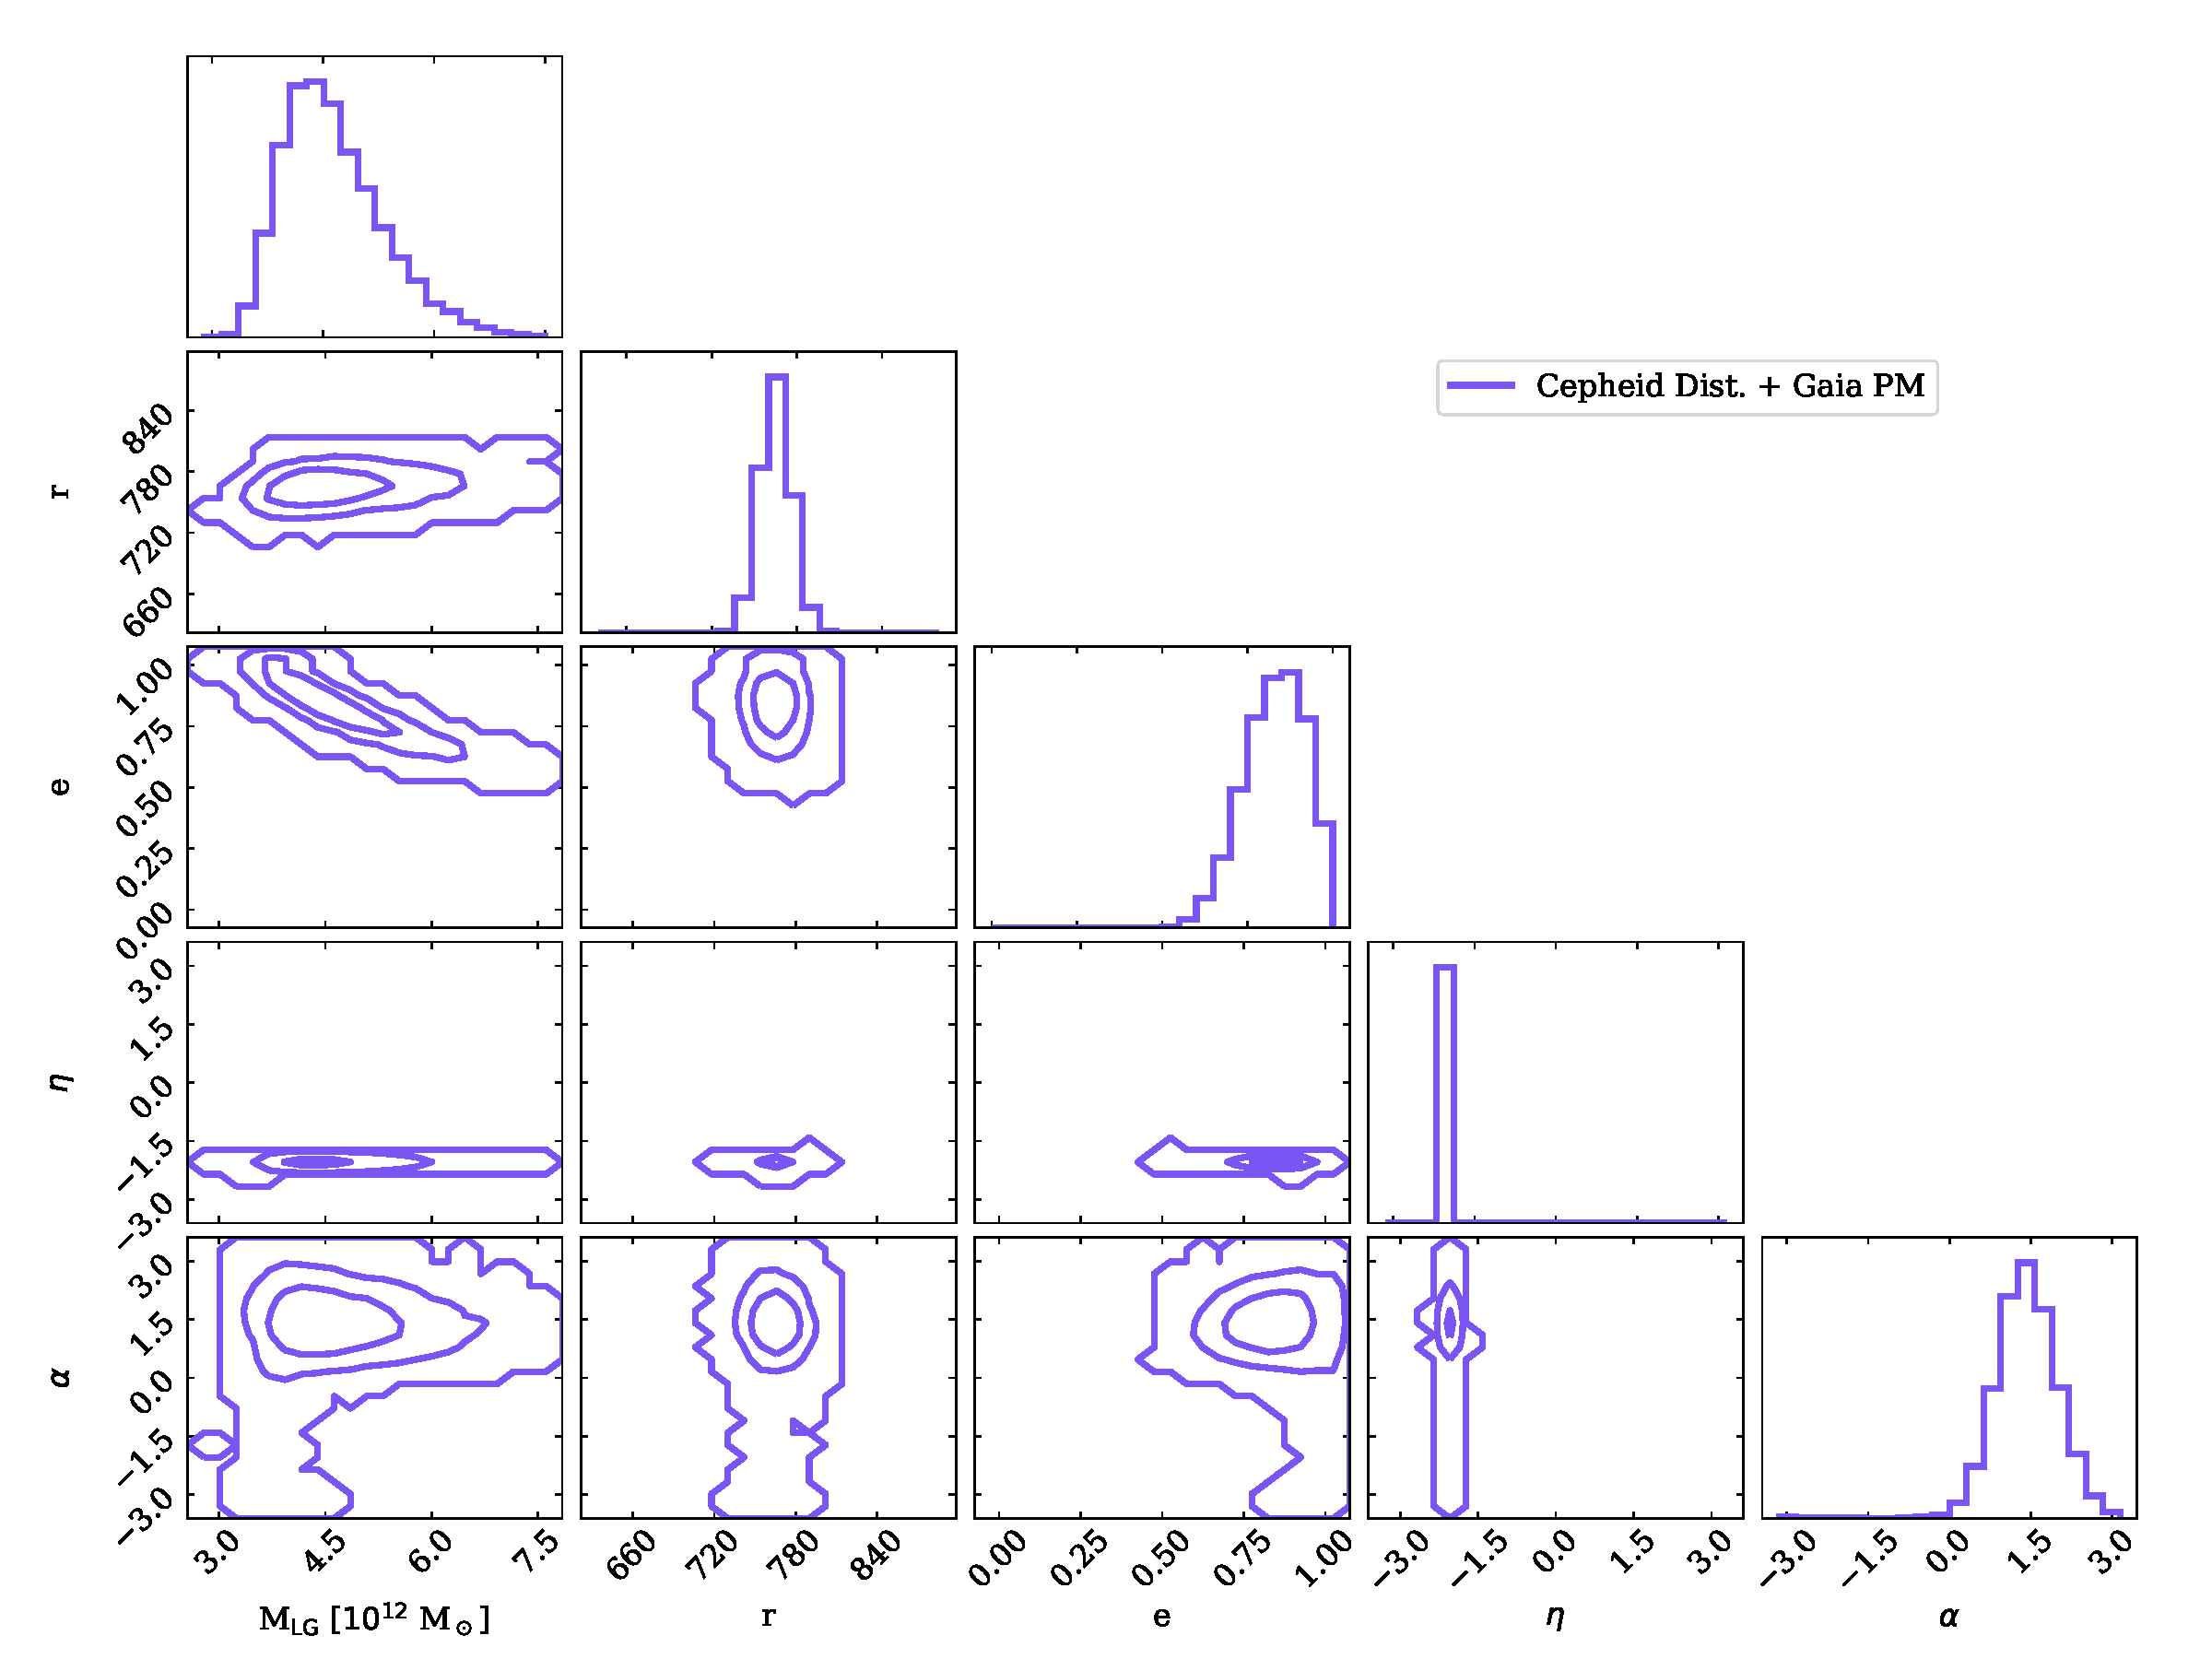
\includegraphics[width=0.8\columnwidth]{analyze-runs-all-fiducial2021.pdf}
  \caption{\label{fig:contour-fiducial}
  68\% and 95\% confidence contours of sampled posterior distributions for all
  model parameters for the cepheid distance
  measurement $761\pm 11 \rm kpc$ and proper motions from \textit{Gaia}.
  }
\end{figure*}

\bibliography{refs}{}
\bibliographystyle{aasjournal}

\end{document}
